\chapter{Model validation and experiments}
\label{ch:experimets}
%Verifica del modello tramite acquisizioni in laboratorio

% APPUNTI
% per verificare il modello, dopo aver tirato fuori l'errore in x e y per ogni punto, ho considerato il fatto che un punto sia in quelle specifiche coordinate come una rv, nella qualle il fatto che il punto sia in quelle due specifiche coordinate è un evento complesso... quindi l'errore complessivo del punto l'ho stimato con la propagazione della varianza $v = v1 + v2 -> std = radq(std1^2 + std2^2)$ \\ poi l'errore nelle misure l'ho stimato come somma dei due errori (propagazione dell'errore lungo differenze) \\ L'idea sarebbe quella di inserire dentro allo stesso modo l'errore sullo speckle si mi dicono che la cosa può avere senso...

\textit{In this chapter we will present the tests performed to understand the effects of subpixel filters in laser peaks detection, and how detected points affect the target final measures. All tests were performed in safety and controlled conditions, using the same industrial lasers that are mounted in the commercial systems. The technology used is entirely produced within the company, thus many information regarding cameras, lasers and measurement systems, will be omitted. For the same reason, only a small part of the scripts we have implemented is available as open source under BSD license \footnote{\url{https://github.com/extoxesses/LaserMat}}.}

% Preliminary phases
  \section{Preliminary phases}
The first set of experiments was partially implemented parallel to model development. This choice allowed us to fully understand each part of the model, and to identify and correct some important errors, not discussed in the previous section. Since the beginning, the main project requirement was to work in limit conditions for the system, in order to analyse each result with respect to the worst case, and determine a lower bound for the system performance. \\

% --- Optical bench
The first thing to do, was to build an optical bench. After many attempts, we made a solid support in which we could fix a laser-camera pair, that allowed us to:
  \begin{itemize}
    \item change the distance between the laser and the camera;
    \item change the triangulation angle, defined as the angle between the optical axis of the camera and the baseline;
    \item change the tilt angle of the lens (only with respect to the $y$ axis)
  \end{itemize}
This first setup was made using a couple of aluminum extrusion profiles, rigidly connected to each other, and a protractor to correctly evaluate the angle of the camera. We used a special case for the camera, that allowed us to set the lens tilt, shielding the sensor from the external light. Furthermore, the case lets to add an interferential filter between the lens and the sensor, cutting all unwanted light frequencies. The laser projection defines a plane parallel to the ground, while the camera looks it from the upside. The accuracy in the distance measurement between the various elements is $1 \, mm$ for the linear distances, and $1 \, degree$ for the angles. The characteristics of the camera and of the laser are shown in Table \ref{tab:conf1}.
  \begin{table}[h!]
  \centering

  \begin{tabular}{ccccc}
    \hline
    \multicolumn{5}{|c|}{\textbf{Camera}}                                                                                                                                                                            \\ \hline
    \multicolumn{1}{|c|}{\textbf{Name}} & \multicolumn{1}{c|}{\textbf{Size}}      & \multicolumn{1}{c|}{\textbf{Pixel size}} & \multicolumn{1}{c|}{\textbf{Lens Manufacturer}} & \multicolumn{1}{c|}{\textbf{Focal}} \\ \hline
    \multicolumn{1}{|l|}{}              & \multicolumn{1}{c|}{\textit{pix x pix}} & \multicolumn{1}{c|}{\textit{$\mu$m}}        & \multicolumn{1}{c|}{}                           & \multicolumn{1}{c|}{\textit{mm}}    \\ \hline
    \multicolumn{1}{|l|}{Spectra}       & \multicolumn{1}{c|}{1710 x 1690}        & \multicolumn{1}{c|}{8.0}                 & \multicolumn{1}{c|}{Linos}                      & \multicolumn{1}{c|}{25}             \\ \hline
    \multicolumn{1}{l}{}                & \multicolumn{1}{l}{}                    & \multicolumn{1}{l}{}                     & \multicolumn{1}{l}{}                            & \multicolumn{1}{l}{}                \\ \cline{2-4}
    \multicolumn{1}{c|}{}               & \multicolumn{1}{c|}{\textbf{Laser}}     & \multicolumn{1}{c|}{}                    & \multicolumn{1}{c|}{}                           &                                     \\ \cline{2-4}
    \multicolumn{1}{c|}{}               & \multicolumn{1}{c|}{\textbf{Frequency}} & \multicolumn{1}{c|}{\textbf{Power}}      & \multicolumn{1}{c|}{\textbf{Aperture}}          &                                     \\ \cline{2-4}
    \multicolumn{1}{c|}{\textit{}}      & \multicolumn{1}{c|}{\textit{nm}}        & \multicolumn{1}{c|}{\textit{W}}          & \multicolumn{1}{c|}{\textit{degree}}            & \textit{}                           \\ \cline{2-4}
    \multicolumn{1}{c|}{}               & \multicolumn{1}{c|}{660}                & \multicolumn{1}{c|}{0.05}                & \multicolumn{1}{c|}{45}                         &                                     \\ \cline{2-4}
  \end{tabular}
  
  \caption{Configuration of the first system.}
  \label{tab:conf1}
\end{table}

% --- The code
\noindent
The second element we needed, was the software. To perform out test, we realized a simple library, written in \textsc{MatLab} \cite{MATLAB:2017}, that implements a calibration algorithm for \acs{SOL} systems, a way to extract the laser from the acquired images, all subpixel filters, described in Section \ref{sec:laser-peaks}, and some scripts to perform our evaluation. Many of these functions were implemented using the \textsc{Image Processing Toolbox}, but many others were implemented from scratch, in order to deeply analyse each operation. The choice to use \textsc{MatLab} was taken for its speed of prototyping and for the type of mathematical operations we are interested in. \\

% --- Calibration process
Once the bench and the software were ready, we had to calibrate the system, and the algorithm we used was Tsai, described in \cite{TsaiTvLenses}. As we  just said, Tsai takes in input a grid of points, both in sensor and in world reference systems, to perform the calibration. To get these points, we tried to use a 2D checkerboard, placed in a plane consistent with the one of the laser. Our idea was to compare the results of Tsai with those of the calibration algorithm in \textsc{MatLab}. So we used two different checkerboards, one with squares size of $9 \, mm$ (shown in Figure \ref{fig:calib1}) and one with squares size of $29 \, mm$. \\
Unfortunately this approach could not work. First of all, the \textsc{Image Processing Toolbox} needed at least two images of the checkerboard, taken in different positions, but it was impossible for us because of the bond on checkerboard position in the laser plane. Furthermore, we observed that, despite our attention in building the system, the laser plane was not completely parallel to the ground one, that means that the checkerboard didn't lie on the same plane of the laser. This introduced another problem: even if we had used Tsai, calibration points would not have met the reality, and our measures will be lost their meanings. Thus, we understood we needed to extend our model, adding laser compensations described with Equations \ref{eq:radial-compensations}, before converting points from the world to the camera. \\

To solve this problem, we decided to use a 3D reference object, of which we know all dimensions, but this type of calibration is pretty different from the previous one. To build the grid of points for Tsai we have to move the target along all the \acs{FOV} of the camera, and to process each acquired frame in order to determine some points of interests. Hence, the target is mounted on a very precise step motor that we move with known steps. In Figure \ref{fig:calib2} we shown a live acquisition of the target: as we can see it is not perpendicular to the optical axis of the camera, that sees something like the one shown in Figure \ref{fig:calib3}. A simple technique to make the grid that we are interested in, is to locate the corner of the holes, as we shown in Figure \ref{fig:calib4}. To detect these points, we need both the frontal and internal profile of the hole: the points will be the intersection of the two line. If we don't have these two information, the diffraction due to laser engraving on the edge of the hole added to many noise to identify the point correctly. Then, if the target was perpendicular to the camera, the inner side wasn't visible. \\
  \begin{figure}[t!]
    \centering
    \begin{minipage}[c]{.48\textwidth}
      \centering
      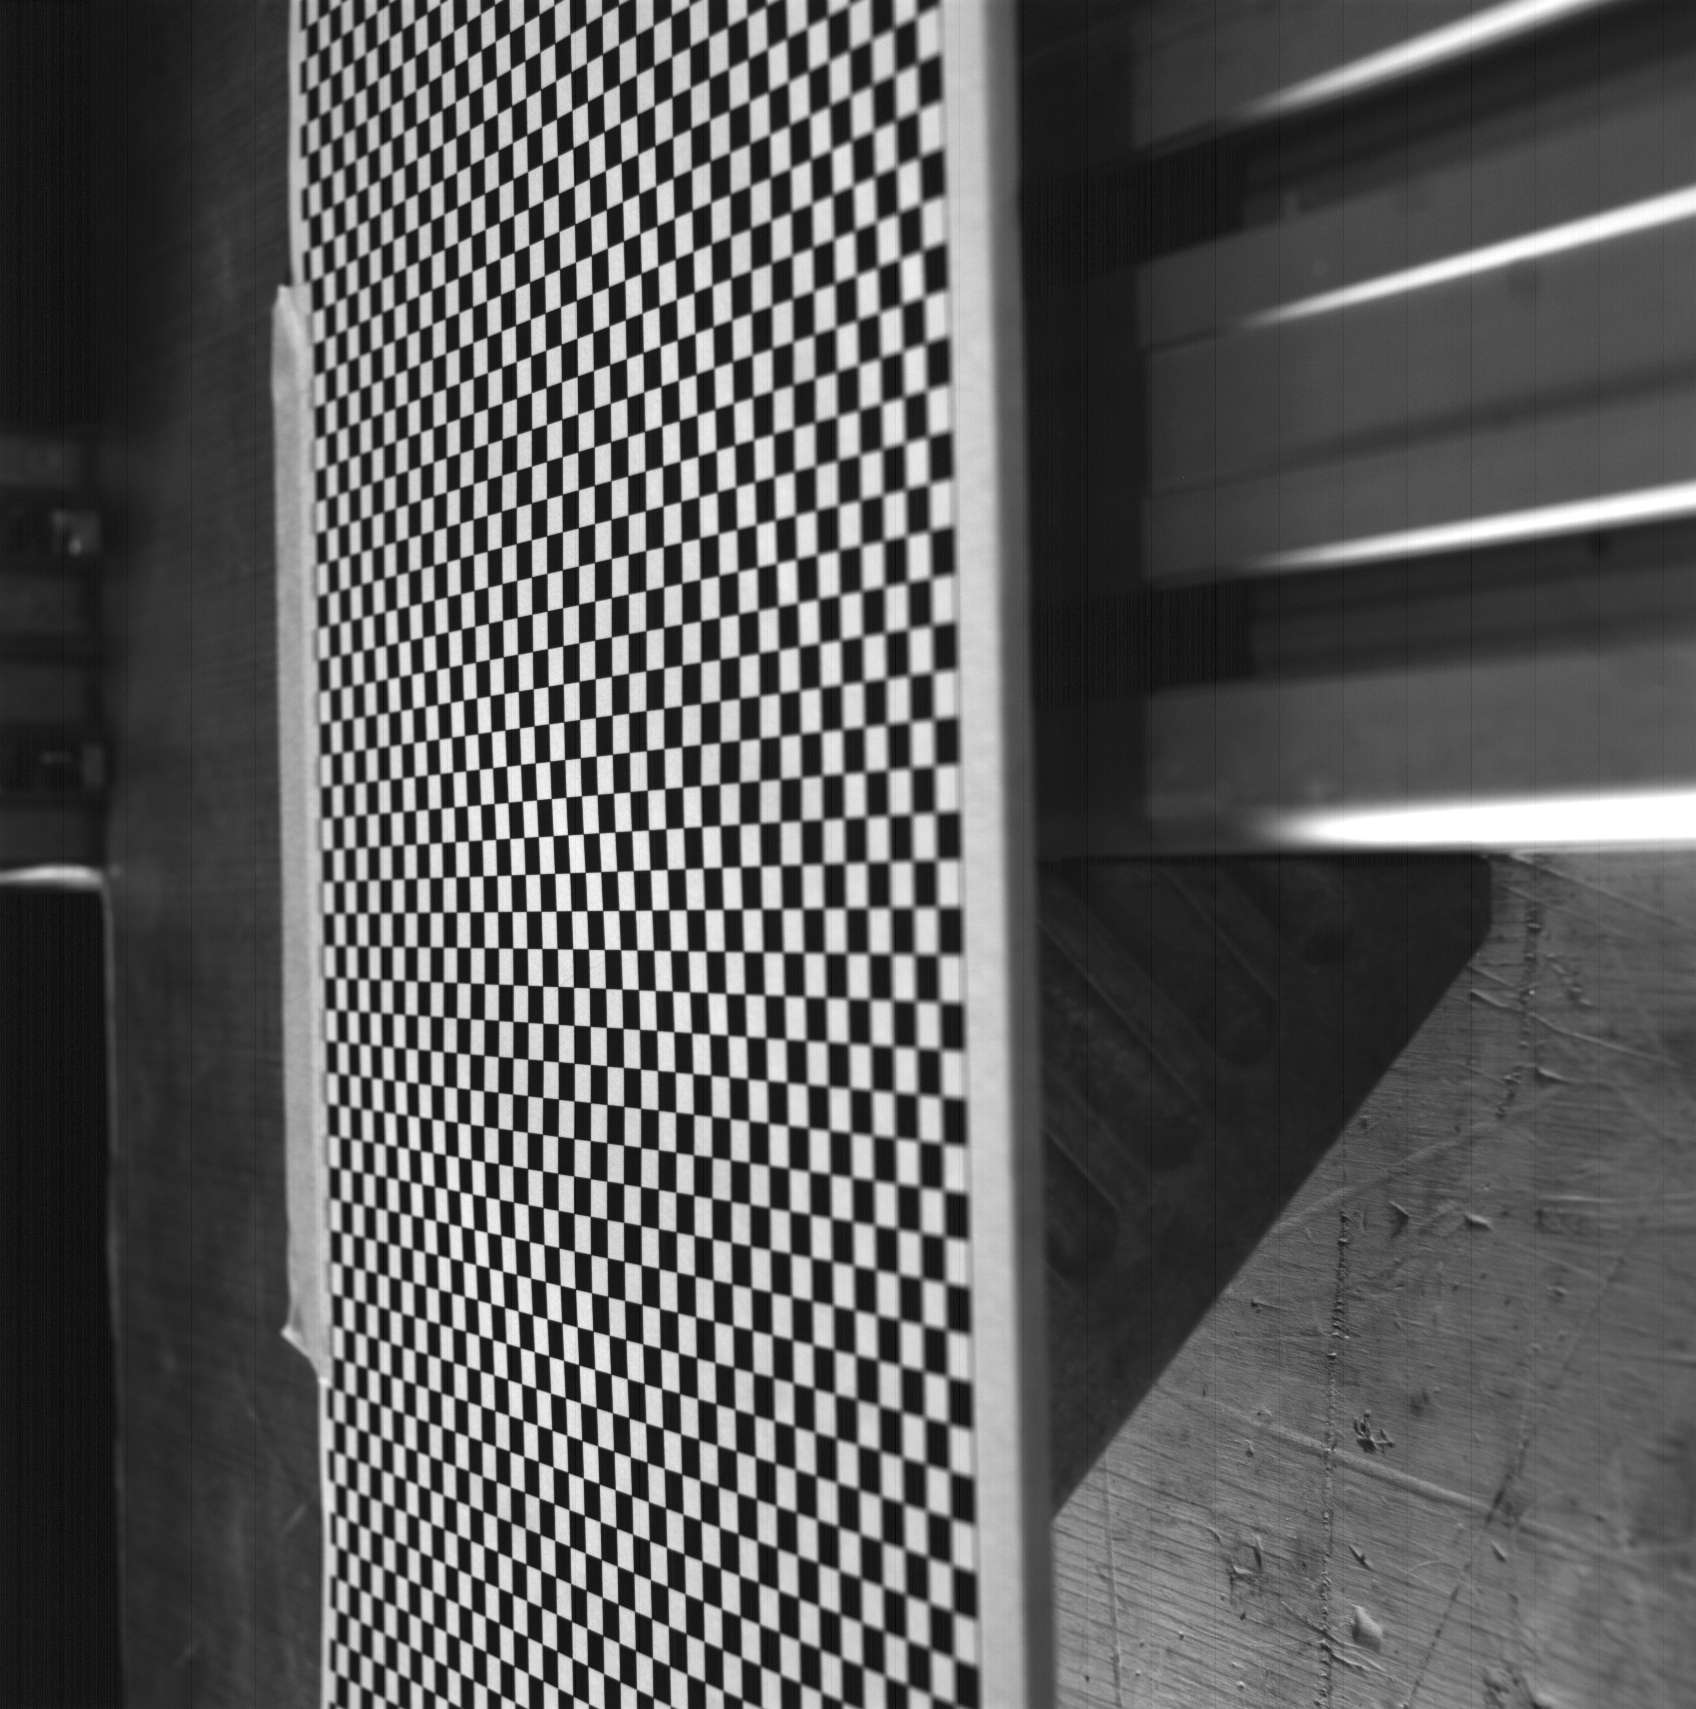
\includegraphics[angle=270, origin=c, width=\textwidth]{./images/analysis/checker09.jpg}
      \caption{Calibration checker with size of squares of $9 \, mm$.}
      \label{fig:calib1}
    \end{minipage}
    \hfill
    \begin{minipage}[c]{.48\textwidth}
      \centering
      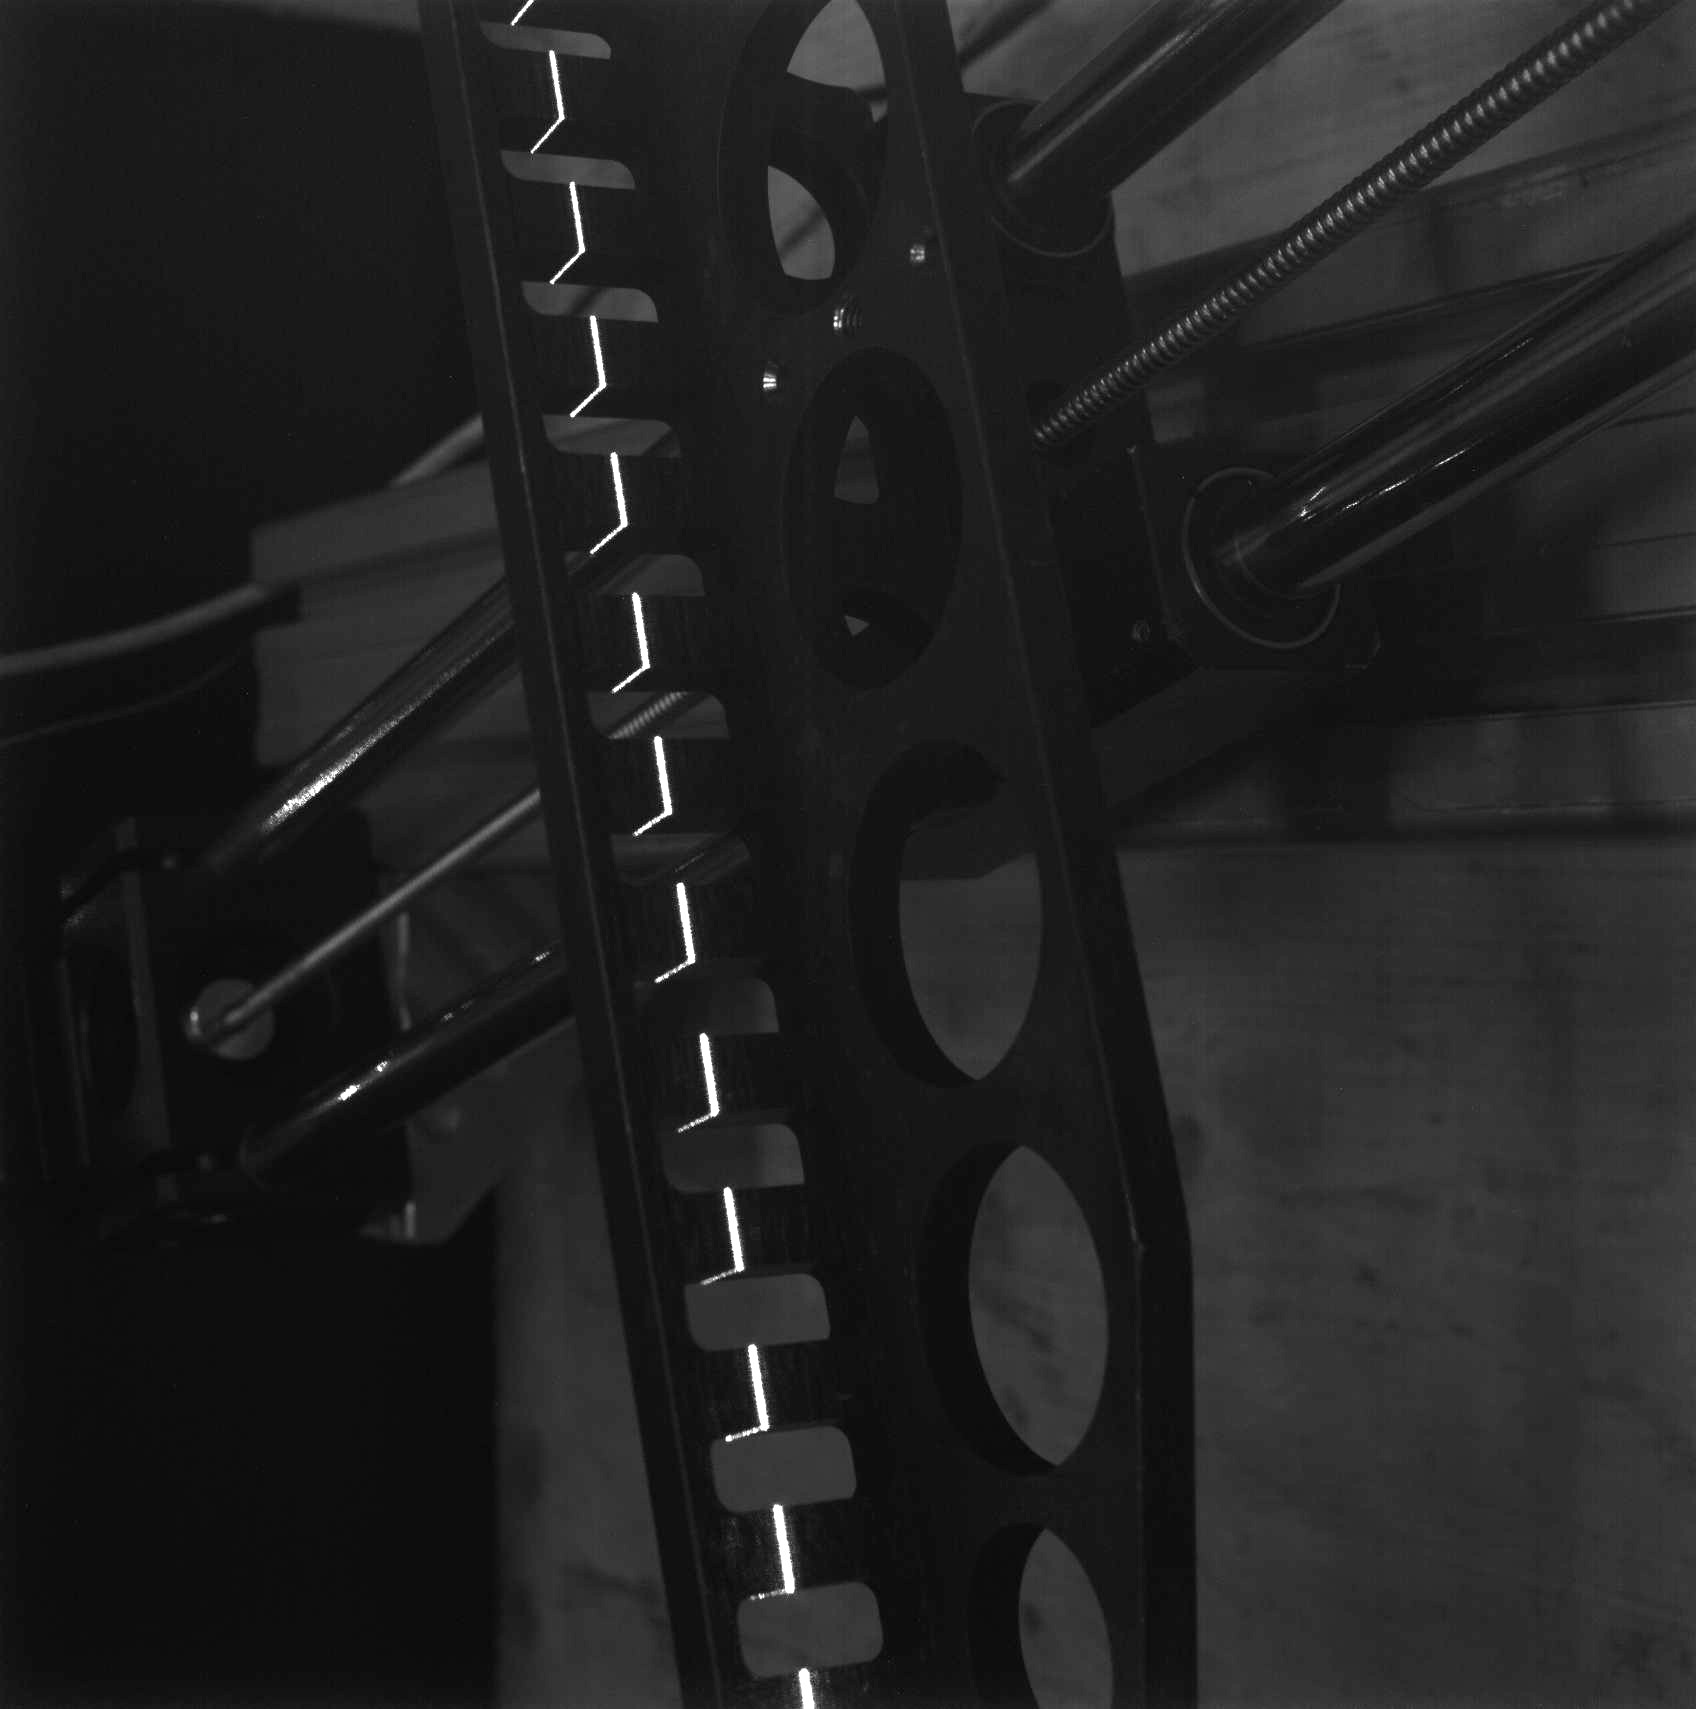
\includegraphics[angle=270, origin=c, width=\textwidth]{./images/analysis/gage.jpg}
      \caption{3D calibration target. \\ ~}
      \label{fig:calib2}
    \end{minipage}
  \end{figure}

  \begin{figure}[t!]
    \begin{minipage}[c]{.48\textwidth}
      \centering
      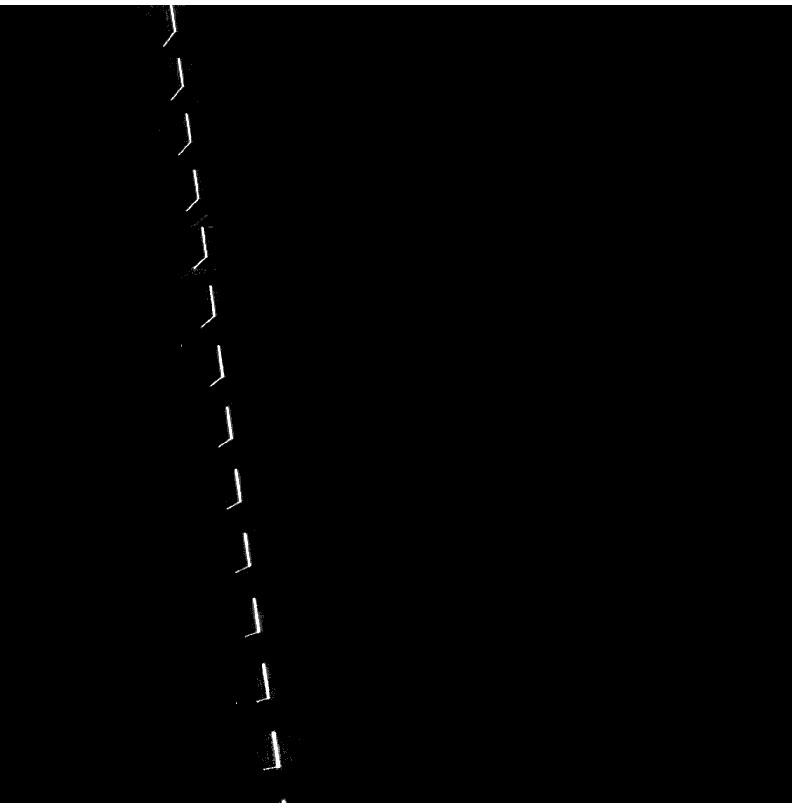
\includegraphics[angle=270, origin=c, width=\textwidth]{./images/analysis/laser_profile_over-gage.jpg}
      \caption{Target profile acquired by the camera.}
      \label{fig:calib3}
    \end{minipage}
    \hfill
    \begin{minipage}[c]{.48\textwidth}
      \centering
      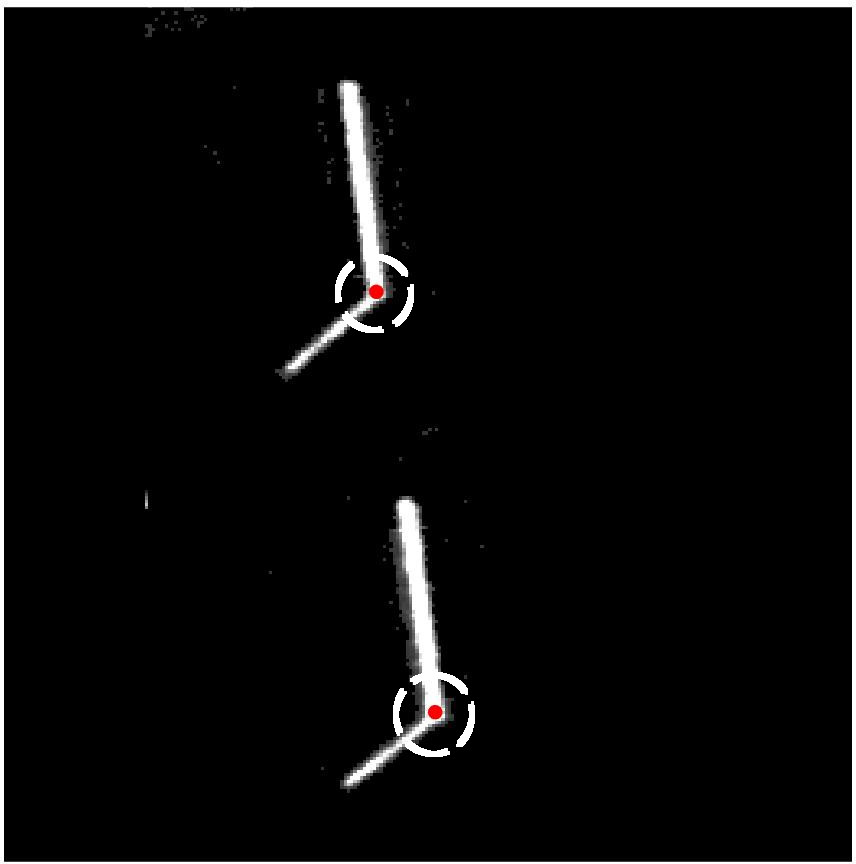
\includegraphics[angle=270, origin=c, width=\textwidth]{./images/analysis/laser_profile_over-gage_corner_det.jpg}
      \caption{Keypoint needed fot the calibration phase.}
      \label{fig:calib4}
    \end{minipage}
  \end{figure}
%    \vfill
%    \begin{minipage}[c]{.48\textwidth}
%      \centering
%      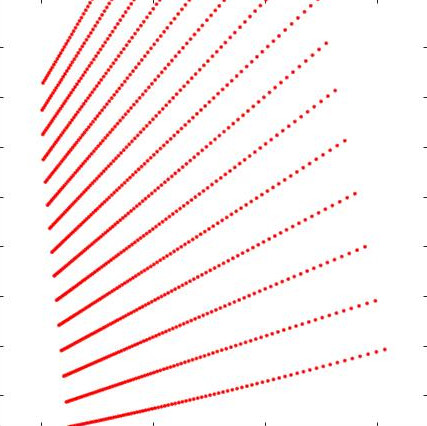
\includegraphics[angle=180, origin=c, width=0.7\textwidth]{./images/analysis/grid.jpg}
%      \caption{Final grid}
%      \label{fig:calib5}
%    \end{minipage}
%    \hfill
%    \begin{minipage}[c]{.48\textwidth}
%      \centering
%      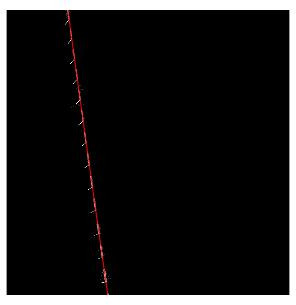
\includegraphics[angle=270, origin=c, width=0.7\textwidth]{./images/analysis/laser_profile_over-gage_fitted.jpg}
%      \caption{Keypoint needed fot the calibration phase.}
%      \label{fig:calib6}
%    \end{minipage}

In the process just described, it is important to consider radial distortion of the lens. What we see in Figure \ref{fig:calib3} is not a straight line, as it is in reality, but because of radial distortion it is a parabola. This mistake leads to the construction of a completely erroneous grid. Another effect of target rotation with respect to the optical axis, is the orientation of the world reference system. This is not a problem, but it is used to apply a correction in order to align the $y$ axis with the \acs{FOV} of the camera, as we assumed in Figure \ref{fig:laser-triang-pdv}. \\

\begin{table}[!t]
  \centering
  \begin{tabular}{@{}cccc@{}}
    \toprule
    \textbf{Measure} & \textbf{Our version}                                                     & \textbf{\textsc{Company version}}                                          & \textbf{Unit}  \\
    \midrule
    $f$ & $36.542$                                                      & $31.971$                                                      & $\left[mm\right]$ \\ && \\
    $k_1$ & $2.24 \cdot 10^{-5}$                                      & $2.3 \cdot 10^{-5}$                                         & $\left[\frac{1}{mm^2}\right]$ \\&& \\
    $T$ & $\begin{bmatrix} 161.605 \\ -35.215 \\ -465.005 \end{bmatrix}$ & $\begin{bmatrix} -157.381 \\ -26.830 \\ 407.198 \end{bmatrix}$ & $\left[mm\right]$ \\&& \\
    $R$ & $\begin{bmatrix}
        -0.770 & -0.638 &  0.015 \\
        -0.415 &  0.482 & -0.772 \\
         0.485 & -0.600 & -0.636 \\
      \end{bmatrix}$ & $\begin{bmatrix}
	     0.765 &  0.644 &  0.009 \\
	     0.480 & -0.562 & -0.673 \\
	    -0.429 &  0.519 & -0.739 \\
      \end{bmatrix}$ & ~ \\ && \\
    $s_x$ & $1$ & $1$ & ~ \\ && \\
    $\left( C_x, C_y \right)$ & $\left(512, 512\right)$                 & $\left(484.387, 918.144\right)$        & $\left[pix\right]$ \\
    \bottomrule
  \end{tabular}
  
  \caption{Comparison between two different version of Tsai's algorithm}
  \label{tab:calib-comparison}
\end{table}
	
In Table \ref{tab:calib-comparison} we compared the results of our implementation of Tsai, with results of a precise implementation, used in industrial systems. The parameters we are interested in are the intrinsic ones. As we can see, the main difference is done by the principal point: in fact, our implementation does not take into account this optimization, so it assumes that the principal point is located in the image center. This is pretty true along the $x$ axis, but not enough along $y$, accordingly with the other version. Furthermore, the difference in focal length is due to the lack of precision of the \textsc{MatLab} optimization functions. \\
As far as extrinsic parameters, however, they depend on the choice of the world reference system that is arbitrarily, thus the sign differences are negligible. From this quick analysis we can concluded not only that our implementation is precise enough for our purposes, but also that the results that we will reach will be a slack lower bounds, that could be improved in real systems implementations. \\

% Fist experiments
  \section{First experiments}
\label{sec:exp1}

In the first set of experiments, we aim to compare our model with the errors made by measuring a well known object, shown in Figure \ref{fig:c5-cad}. The target was made with a \acs{CNC} machine with a precision of $0.1 \, mm$ with respect to all the measures reported in Figure \ref{fig:c5-cad-misure}. Our goal was to reach this measurement precision. \\

The point cloud obtained with our algorithm is shown in Figure \ref{fig:c5-profile_pixel}: the points are plotted in the world reference system, after that we have projected the laser spots, detected in the image.

\begin{figure}
  \begin{minipage}[c]{.44\textwidth}
    \centering
    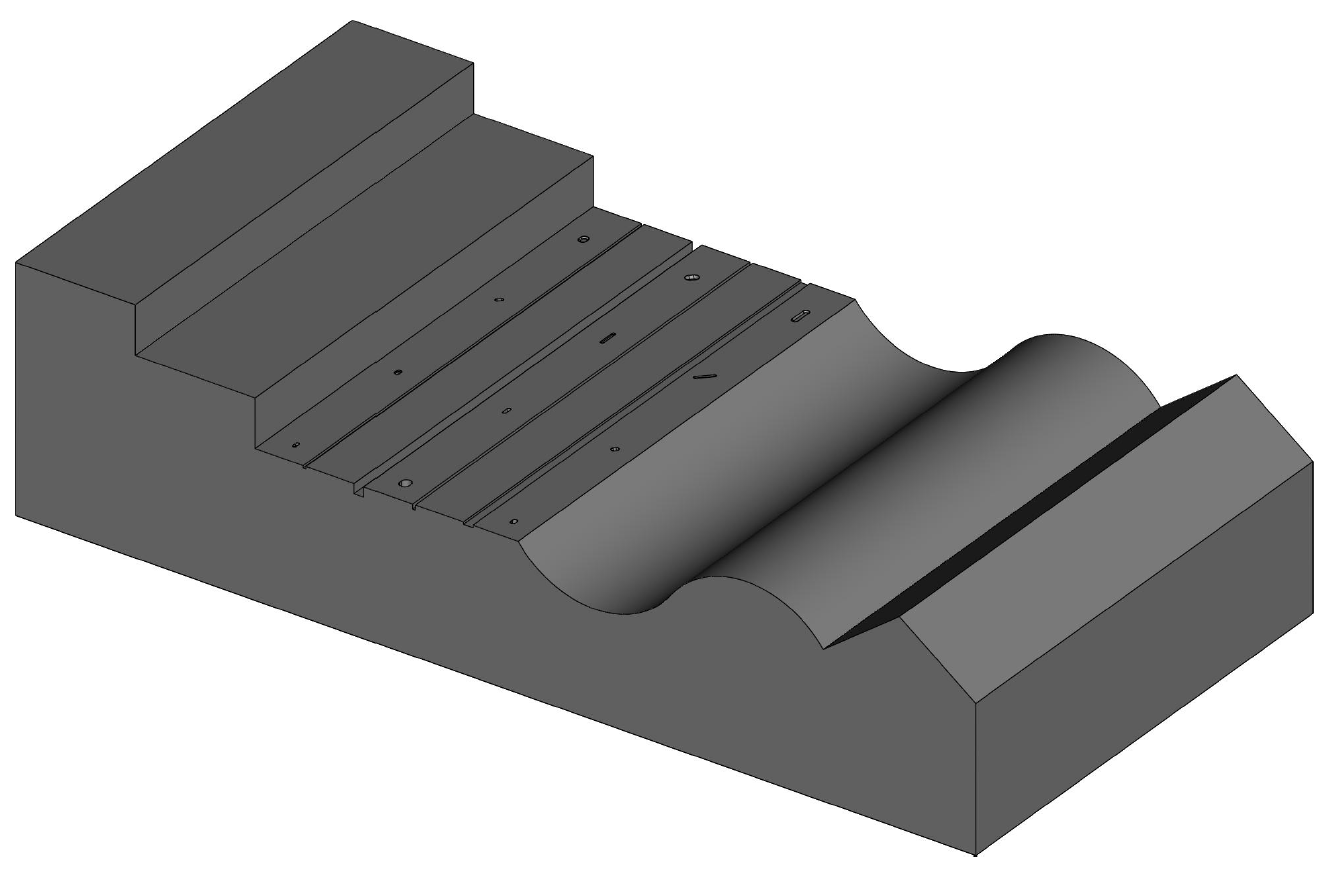
\includegraphics[width=\textwidth]{./images/analysis/t1/cad.png}
    \caption{CAD of the target \\ object}
    \label{fig:c5-cad}
  \end{minipage}
  \hfill
  \begin{minipage}[c]{.55\textwidth}
    \centering
    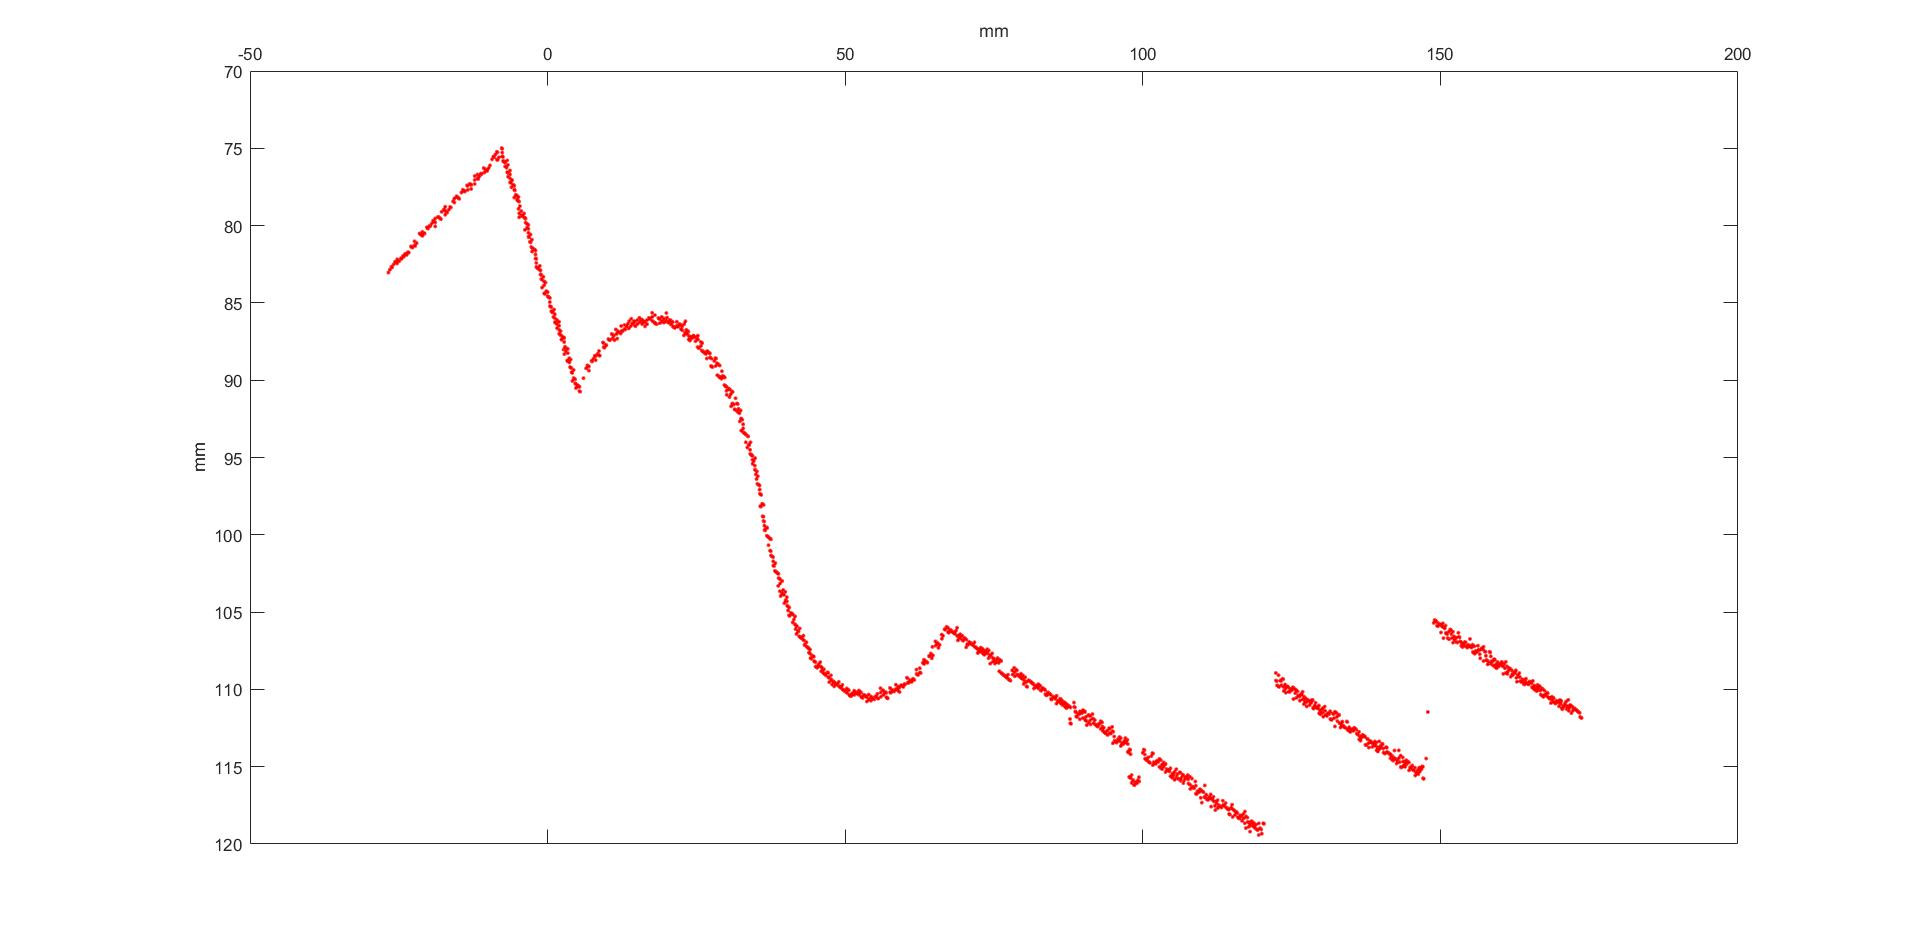
\includegraphics[width=\textwidth]{./images/analysis/t1/pixel_profile_cut.jpg}
    \caption{Laser spots, complete profile}
    \label{fig:c5-profile_pixel}
  \end{minipage}
\end{figure}
\vfill
\begin{figure}
  \centering
  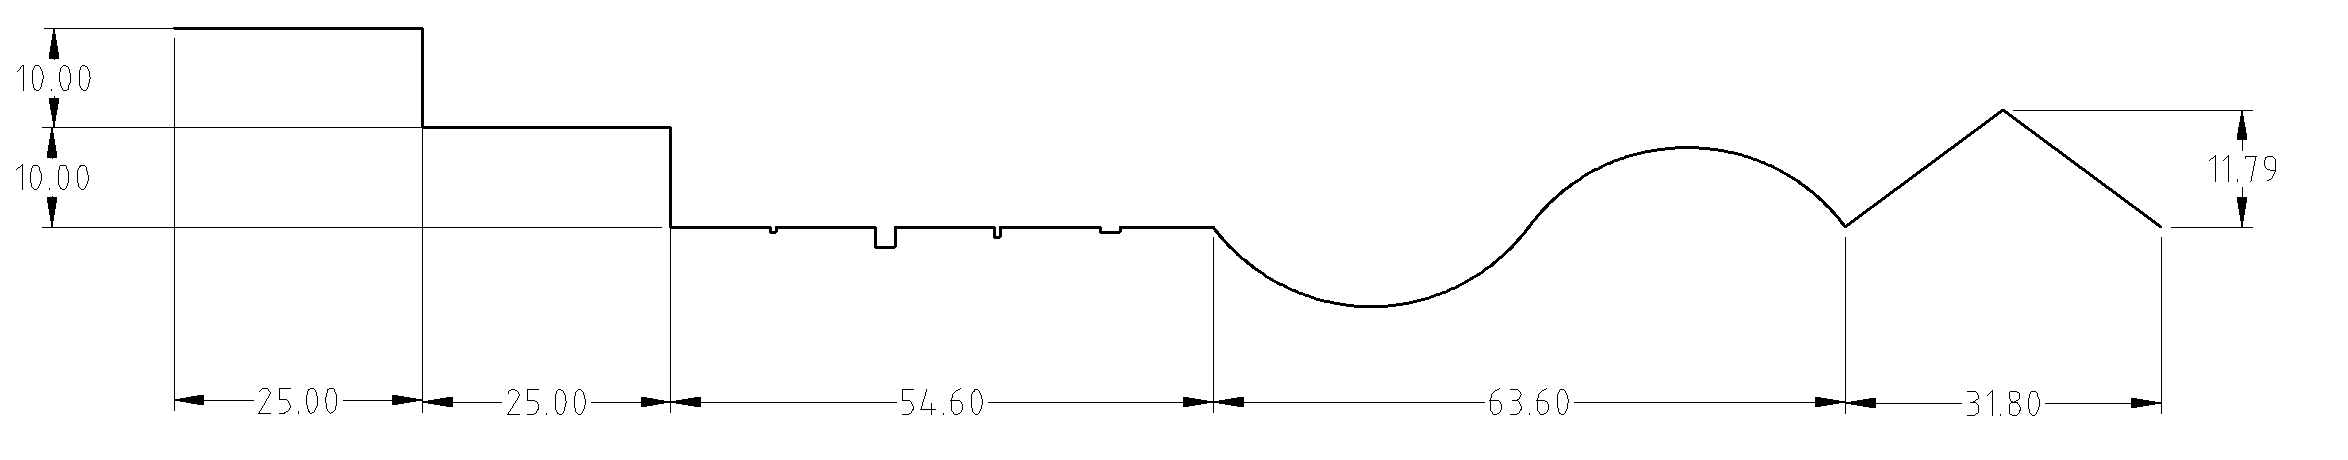
\includegraphics[width=\textwidth]{./images/analysis/t1/cad_misure.png}
  \caption{Measures of the target object}
  \label{fig:c5-cad-misure}
\end{figure}
\vfill
\begin{figure}
  \centering
  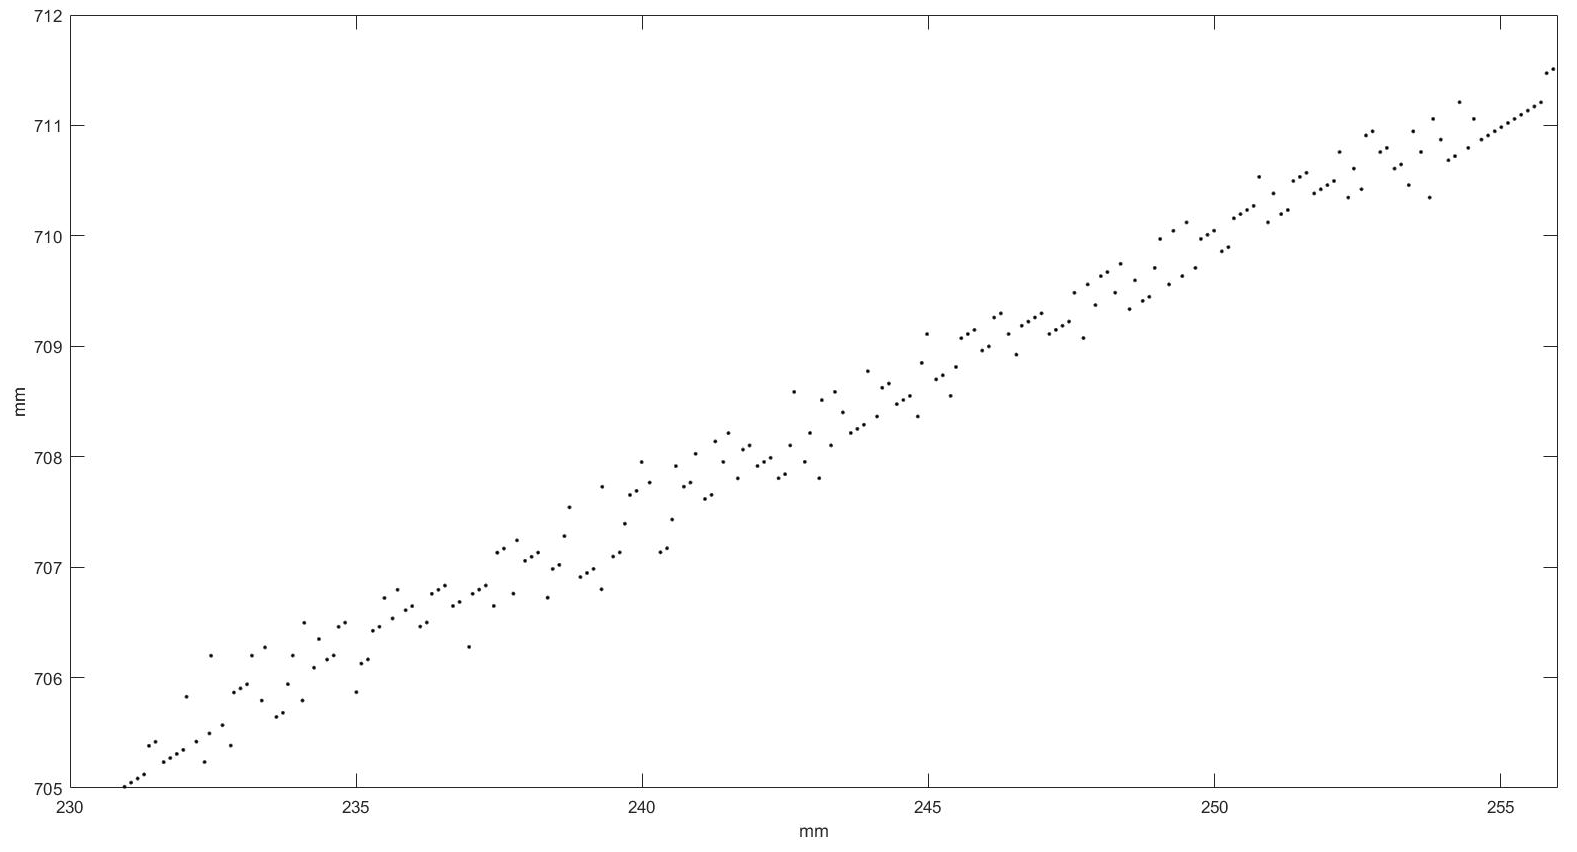
\includegraphics[width=\textwidth]{./images/analysis/t1/pixel_profile_det.jpg}
  \caption{Details of the laser spots}
  \label{fig:c5-profile_pixel_det}
\end{figure}
\vfill
\begin{figure}
  \centering
  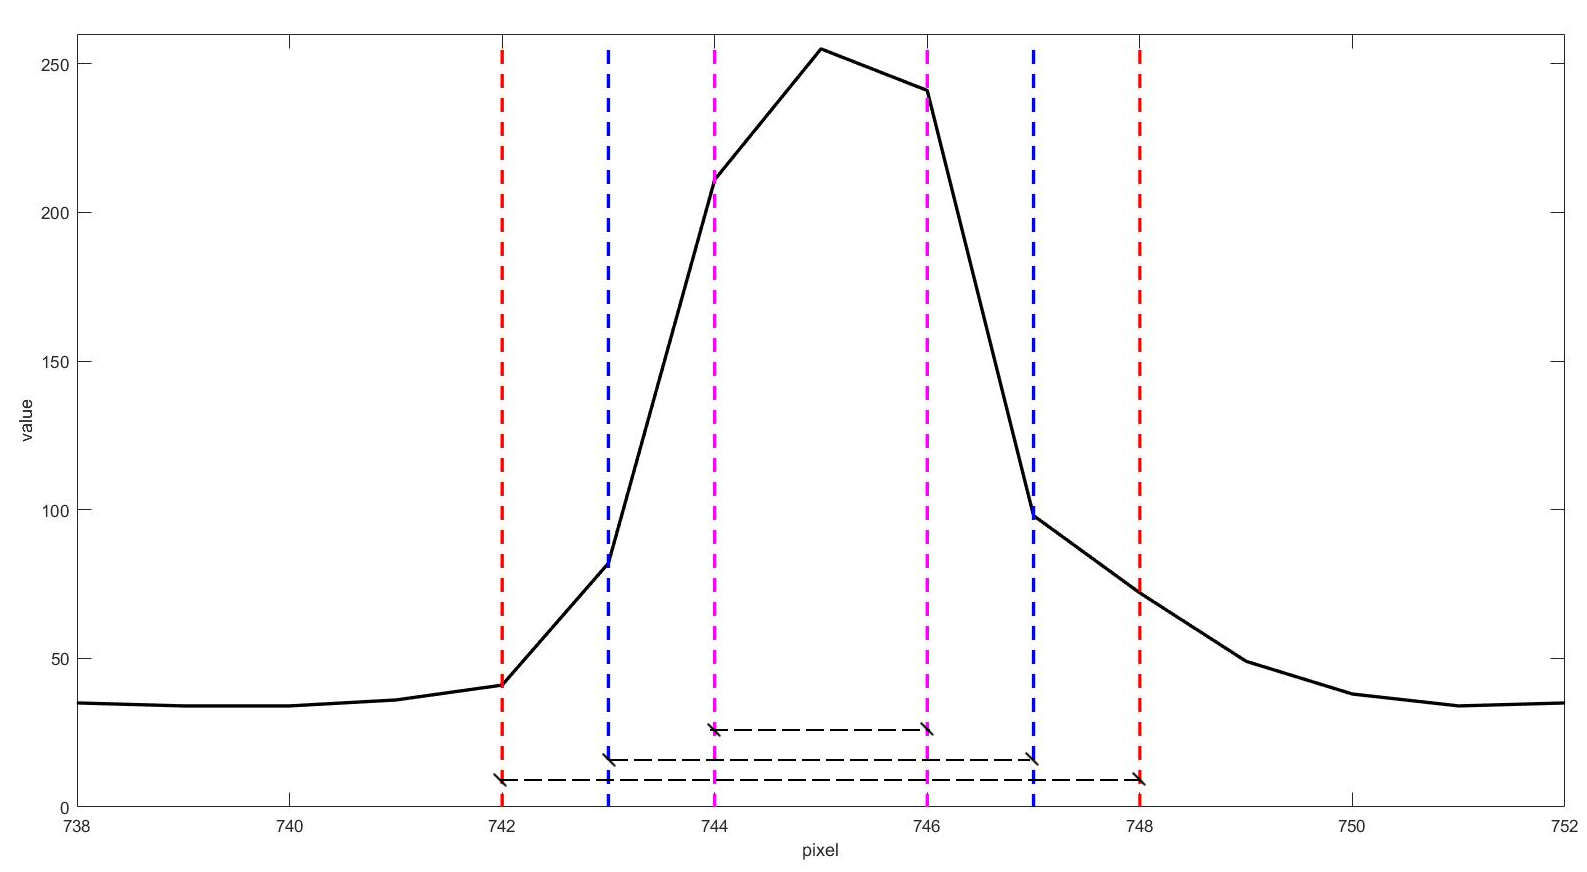
\includegraphics[width=\textwidth]{./images/analysis/t1/peak_distrib.jpg}
  \caption{Distribution of the energy along a row of the image. Vertical lines indicate the 3 windows used.}
  \label{fig:c5-peak_distrib}
\end{figure}
\vfill
\begin{figure}
  \centering
  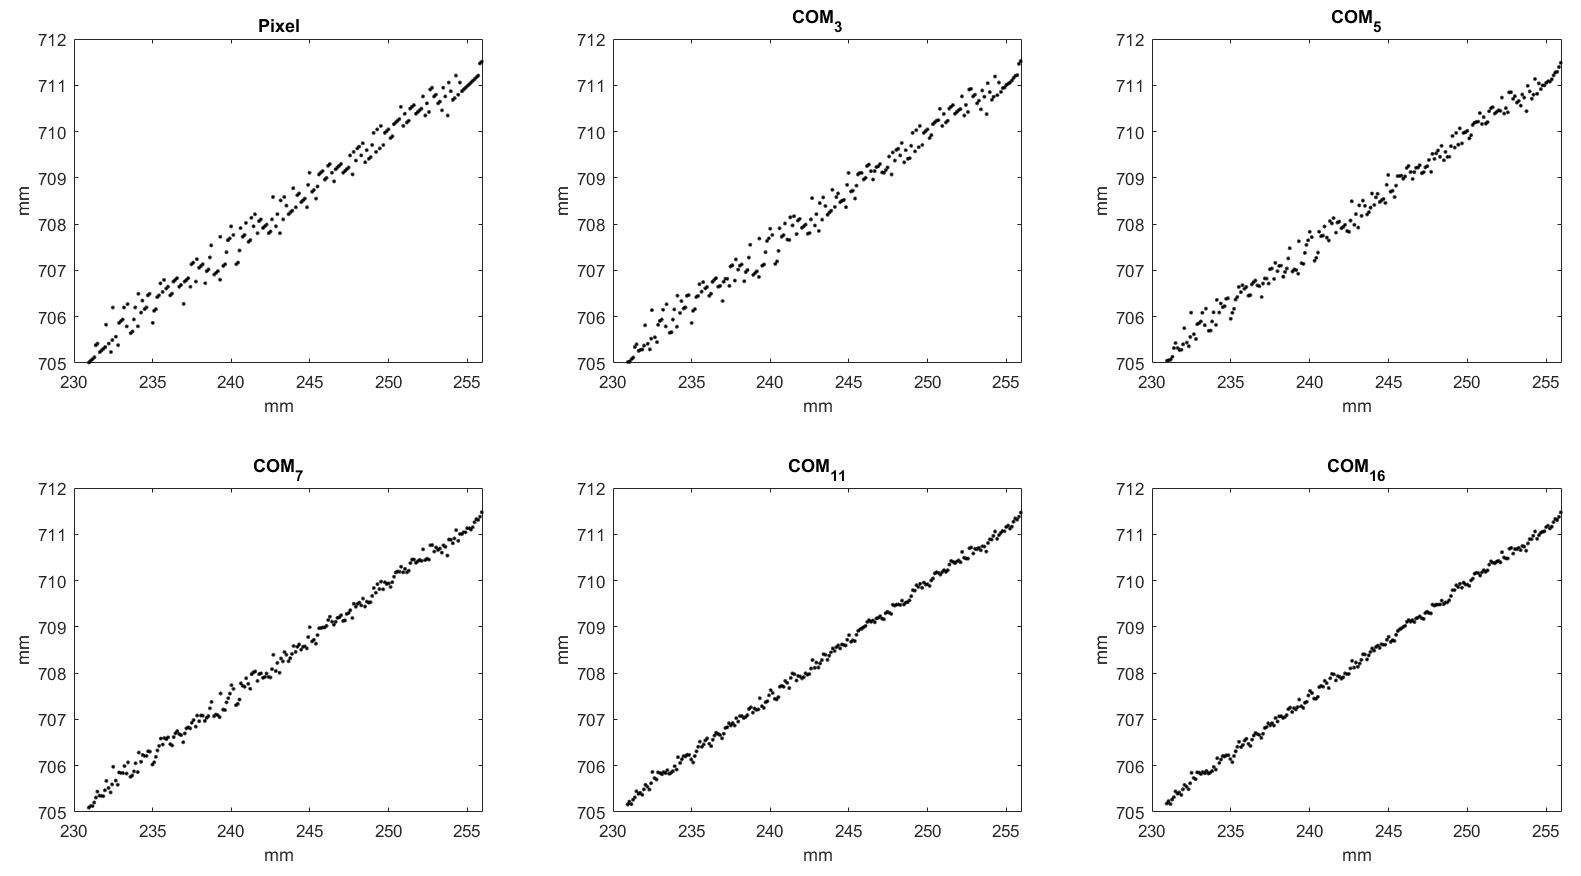
\includegraphics[width=\textwidth]{./images/analysis/t1/com6_cmp.jpg}
  \caption{Comparison of \textit{Center of Mass} applied with extended widow sizes}
  \label{fig:c5-com_cmp_6}
\end{figure}
\vfill
\begin{figure}
  \centering
  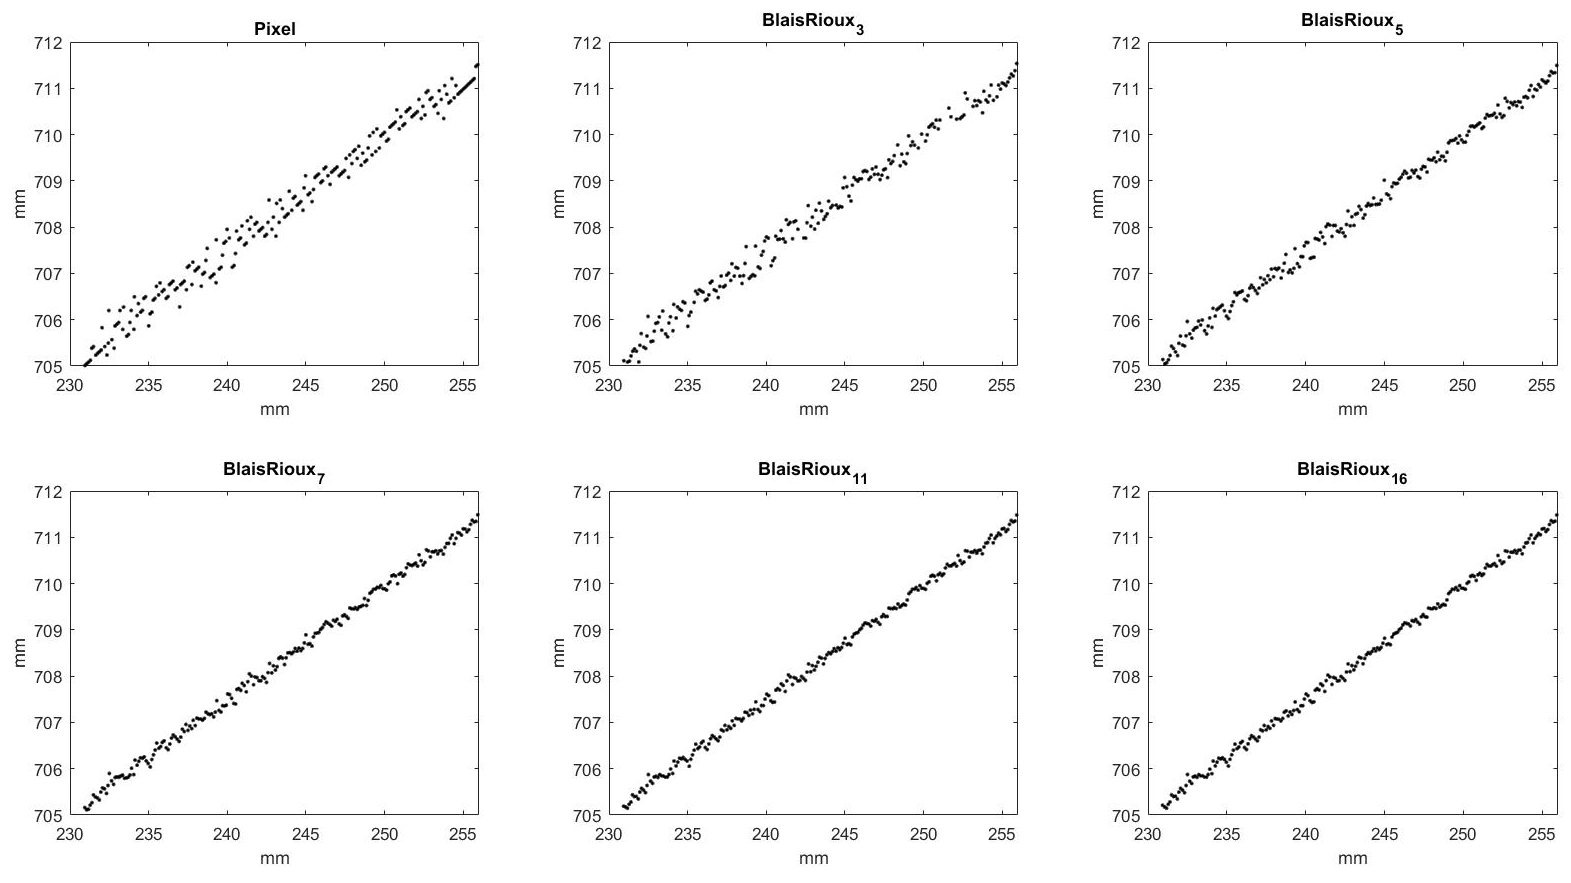
\includegraphics[width=\textwidth]{./images/analysis/t1/br6_cmp.jpg}
  \caption{Comparison of \textit{Blais and Rioux} applied with extended widow sizes}
  \label{fig:c5-br_cmp_6}
\end{figure}
\begin{figure}
  \centering
  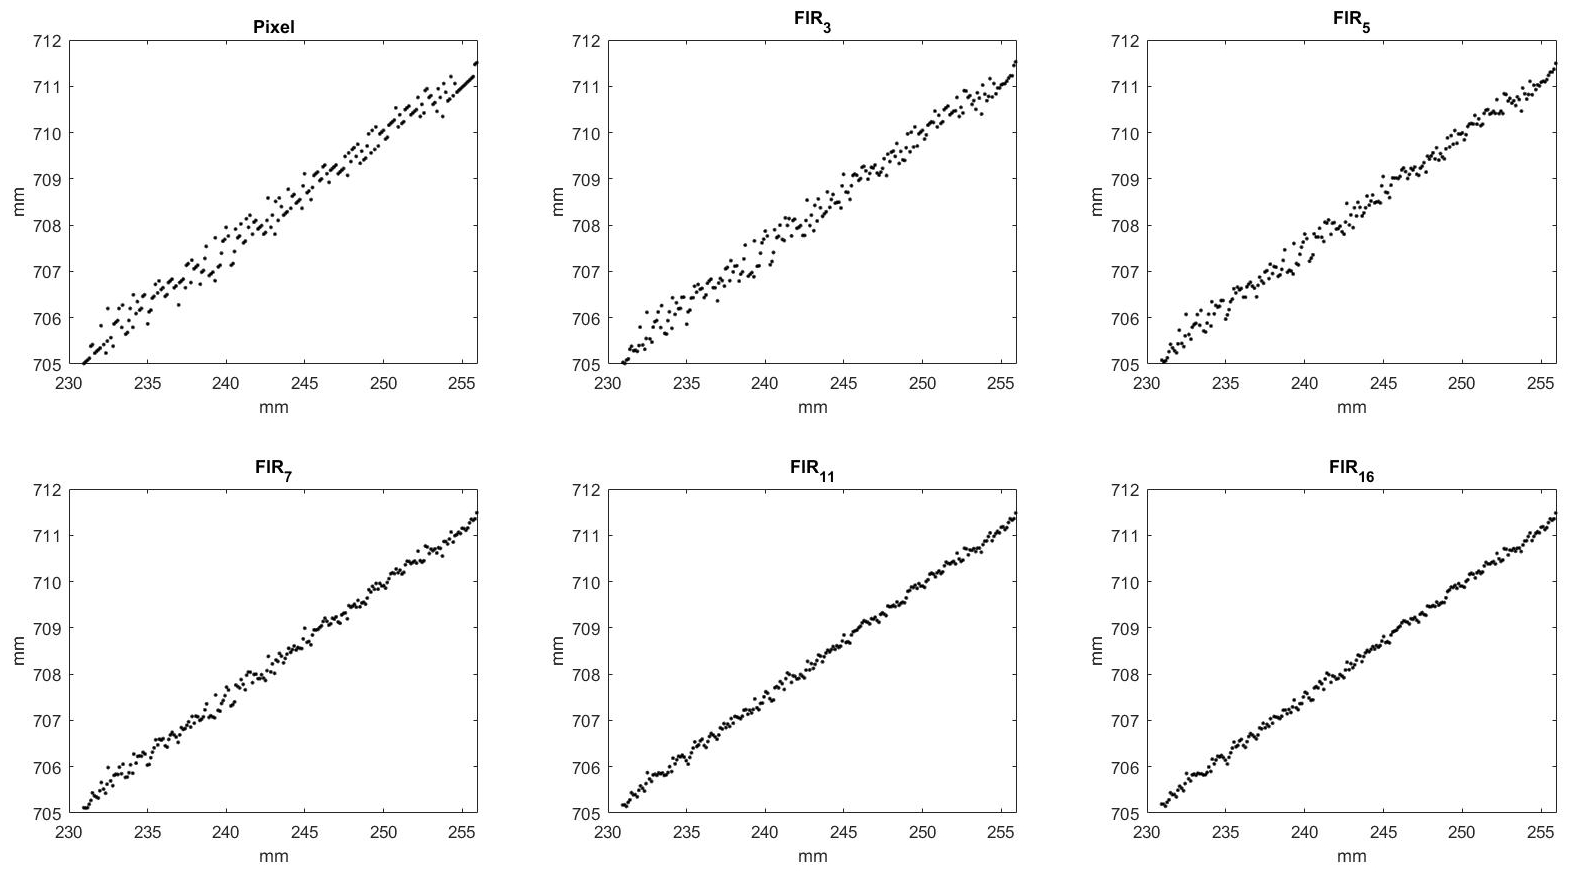
\includegraphics[width=\textwidth]{./images/analysis/t1/fir6_cmp.jpg}
  \caption{Comparison of \textit{FIR} applied with extended widow sizes}
  \label{fig:c5-fir_cmp_6}
\end{figure}
\clearpage

If we magnify the data, as shown in Figure \ref{fig:c5-profile_pixel_det}, we can observe that the acquired profile is very thick. This effect is due to the noise of the laser beam (e.g. speckle), that causes small variations of the positions of the peaks, along a line of the image. Thus, we expected that the use of sub-pixel filters, should reduce the thickness of the beam. All the model described in Section \ref{sec:laser-peaks}, were introduced considering only few pixel around the candidate to be the peak. So we tried to apply them, using windows of $3$, $5$ and $7$ pixel were possible. \\

Unfortunately, the results made us wrong. Observing the live images, we noticed that the width of the Gaussian was on average equal to $20$ pixels, as the row shown in Figure \ref{fig:c5-peak_distrib}: the used interval are too small with respect to signal amplitude. Hence, we decided to increase the window to $11$ and $16$ pixels where possible. In Figure \ref{fig:c5-com_cmp_6} we can see the improvement of the detail shown in Figure \ref{fig:c5-profile_pixel_det}, obtained using the \textit{center of mass}. Therefore, we concluded that, in order to get a sufficiently precise smoothing, it is necessary that the window is bigger enough to contain the whole laser spot. To complete our analysis, we tried to further increase the size of the window. This tests did not lead to significant improvements over the windows of $11$ or $16$ pixels. On the contrary in some cases, for example in noisy areas of the images, or because the background noise, the use of a larger window deteriorated the peak recognition. \\
We reached the same results analysing the remaining filters, as shown in Figures \ref{fig:c5-br_cmp_6} and \ref{fig:c5-fir_cmp_6}. From these observations, we concluded that the windows sizes have to be comparable with the Gaussian: if they are too small, the profile will be less precise; if they are too big, we risk to add noise.

Regarding the remaining filters (Gaussian, Linear and Parabolic), we have found some difficulties extending them, in order to increase the number of points involved in: as we have already said, $3$ pixels are too few to obtain a good approximation of the laser beam. However, this operation has proved to be meaningless. The three models are based on weighted linear models, such that they work properly only if three pixel are used. Change these weights, changes the meaning of the model itself. The only one that has been extended (the Parabolic) did not reach the results reached with the \textit{\acs{COM}}, the \textit{Blaise\&Rioux} or with the \textit{FIR} filter. Thus, we decided to ignore them from our analysis.

A second observation in support of this choice is due to the saturation effect. Sometimes could happen that some consecutive pixels have the same (maximum) value, caused by changing in the illumination of the working place, out of focus lenses or lasers, or caused by translucid or labertian surfaces. If we use only $3$ or $4$ pixels, it is impossible for these filters to properly identify the peak the the laser spot. \\
  
At this point, we were able to evaluate some measures. To simplify the task, we decided to consider a few well-recognizable points of the profile, i.e. the points used in Figure \ref{fig:c5-cad-misure} to add quotes. Thus, we used a simple 3D corner detector, and the measures were computed as differences between the points, after the alignment of the detected profile to the model. \\
Before achieving remarkable results, we found some difficulties. The most important, is related to calibration. As we said in Section \ref{sec:teo-calibration}, it is fundamental that the grid of calibration points covers the entire \acs{FOV} of the camera. Despite that, the points have to be always on focus. If for any reasons this condition is not true, some of these points could affect the quality of the calibration itself. Thus, we manually reduced the grid until we reached a tiny type I error. \\

Finally, we had got the first results. In Figure \ref{fig:c5-match} we shown the match computed before estimate the measures, while in Tables \ref{tab:c5-r1-teo} and \ref{tab:c5-r1-real} we reported an example of how we estimated the measurement error (theoretically and with empirical data), in particular these results are obtained using the \textit{center of mass} with a window of $16$ pixels. Note that, in order to evaluate column \textit{point error}, we assumed that the event that a point falls in $p = (x, y)$ can be modelled as the union of two i.i.d. events, followed by:
  \begin{equation}
    \sigma_p = \sqrt{\sigma_x^2 + \sigma_y^2}
    \label{eq:exp:var-prop}
  \end{equation}
  \begin{figure}[t!]
    \centering
    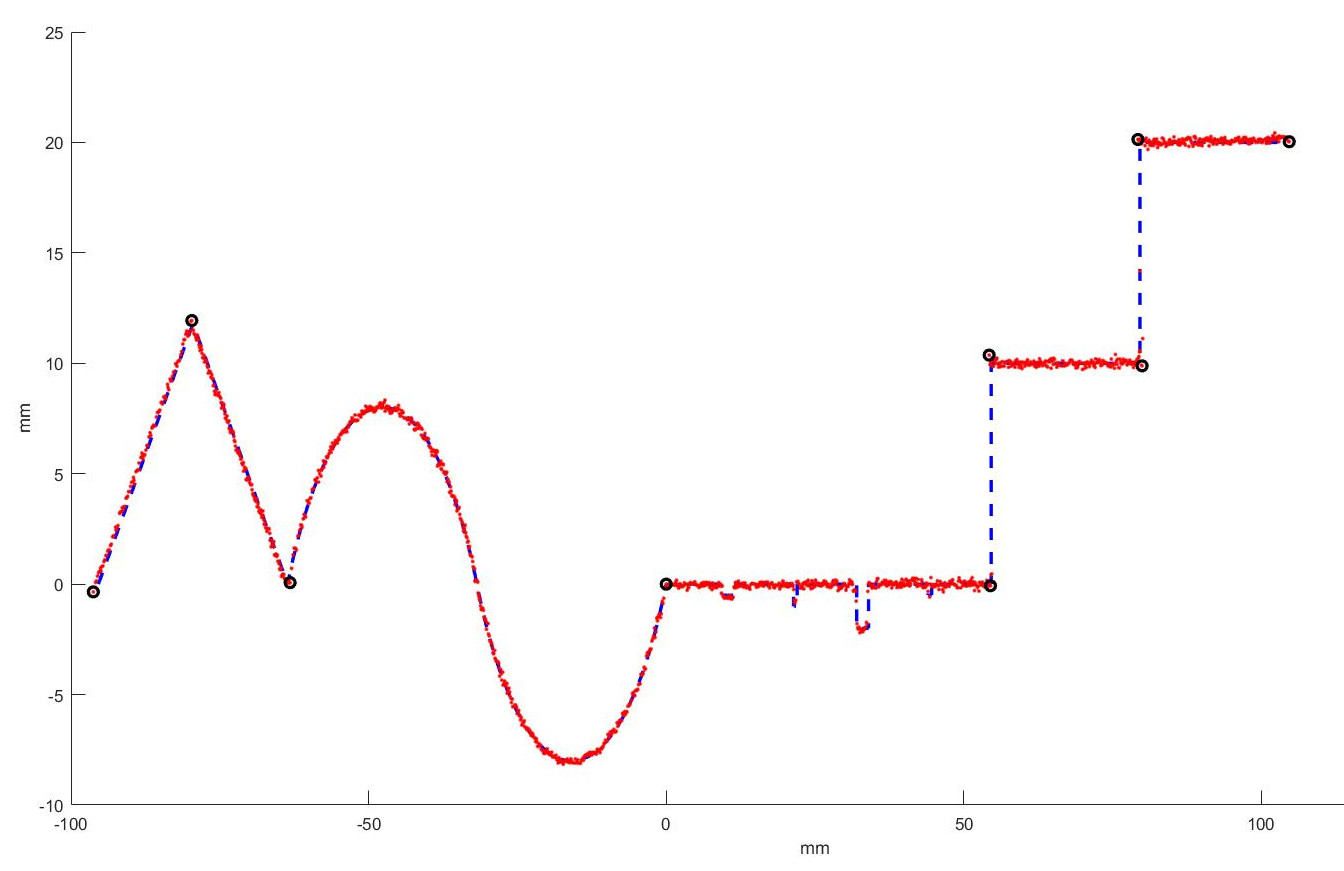
\includegraphics[width=\textwidth]{./images/analysis/t1/example_cut.jpg}
    \caption{Example of match of the profile extracted using \textit{center of mass} with window of $16$ pixel. The model is plotted in blue, while the extracted profile is plotted in red.}
    \label{fig:c5-match}
  \end{figure}
  \begin{table}[b!]
\centering
\begin{tabular}{|r|r|r|r|}
\hline
\multicolumn{1}{|c|}{\textbf{Approximation}} & \multicolumn{1}{c|}{\textbf{Y Error}} & \multicolumn{1}{c|}{\textbf{X Error}} & \multicolumn{1}{c|}{\textbf{Point Error}} \\ \hline
\multicolumn{1}{|c|}{\textit{(pix)}}           & \multicolumn{1}{c|}{\textit{(mm)}}      & \multicolumn{1}{c|}{\textit{(mm)}}      & \multicolumn{1}{c|}{\textit{(mm)}}          \\ \hline
0.1089                                       & 0.0153                                & 0.5678                                & 0.5680                                    \\ \hline
0.1089                                       & 0.0101                                & 0.3261                                & 0.3263                                    \\ \hline
0.1089                                       & 0.0073                                & 0.6246                                & 0.6246                                    \\ \hline
0.1089                                       & 0.0095                                & 0.7877                                & 0.7877                                    \\ \hline
0.1089                                       & 0.0528                                & 0.9875                                & 0.9889                                    \\ \hline
0.1089                                       & 0.0534                                & 0.6900                                & 0.6921                                    \\ \hline
0.1089                                       & 0.1157                                & 0.8070                                & 0.8152                                    \\ \hline
0.1089                                       & 0.1172                                & 0.4760                                & 0.4902                                    \\ \hline
0.1089                                       & 0.2220                                & 0.5741                                & 0.6155                                    \\ \hline
\multicolumn{3}{|r|}{\textbf{Mean}}                                                                                          & \textbf{0.6565}                           \\ \hline
\end{tabular}
\caption{Theoretical results obtained using the \textit{Center of Mass} with window of 16 pixel}
\label{tab:c5-r1-teo}
\end{table}
  \begin{table}[h!]
\centering
\begin{tabular}{|r|r|r|r|r|r|r|}
\hline
\multicolumn{3}{|c|}{\textbf{Abscissa}}                                                                             & \multicolumn{3}{c|}{\textbf{Ordinate}}                                                                             & \multicolumn{1}{c|}{\multirow{2}{*}{\textbf{Point Error}}} \\ \cline{1-6}
\multicolumn{1}{|c|}{\textbf{Model}} & \multicolumn{1}{c|}{\textbf{Profile}} & \multicolumn{1}{c|}{\textbf{Errors}} & \multicolumn{1}{c|}{\textbf{Model}} & \multicolumn{1}{c|}{\textbf{Profile}} & \multicolumn{1}{c|}{\textbf{Errors}} & \multicolumn{1}{c|}{}                                      \\ \hline
\multicolumn{1}{|c|}{\textit{(mm)}}           & \multicolumn{1}{c|}{\textit{(mm)}}      & \multicolumn{1}{c|}{\textit{(mm)}}      & \multicolumn{1}{c|}{\textit{(mm)}} & \multicolumn{1}{c|}{\textit{(mm)}}      & \multicolumn{1}{c|}{\textit{(mm)}}      & \multicolumn{1}{c|}{\textit{(mm)}}          \\ \hline
15.9010                              & 16.5450                               & 0.6438                               & 11.7920                             & 12.2720                               & 0.4804                               & 0.8033                                                     \\ \hline
15.9000                              & 16.5160                               & 0.6157                               & 11.7920                             & 11.8430                               & 0.0511                               & 0.6178                                                     \\ \hline
63.6000                              & 63.1840                               & 0.4159                               & 0.0000                              & 0.0909                                & 0.0909                               & 0.4257                                                     \\ \hline
54.6000                              & 54.4860                               & 0.1144                               & 0.0000                              & 0.0863                                & 0.0863                               & 0.1433                                                     \\ \hline
0.0000                               & 0.2235                                & 0.2235                               & 10.0000                             & 10.4530                               & 0.4530                               & 0.5051                                                     \\ \hline
25.0000                              & 25.6950                               & 0.6949                               & 0.0000                              & 0.5067                                & 0.5067                               & 0.8600                                                     \\ \hline
0.0000                               & 0.7019                                & 0.7019                               & 10.0000                             & 10.2750                               & 0.2746                               & 0.7537                                                     \\ \hline
25.0000                              & 25.4190                               & 0.4189                               & 0.0000                              & 0.1010                                & 0.1010                               & 0.4309                                                     \\ \hline
\multicolumn{6}{|r|}{\textbf{Mean}}                                                                                                                                                                                                      & \textbf{0.5675}                                            \\ \hline
\end{tabular}
\caption{Results obtained using the \textit{Center of Mass} with window of 16 pixel}
\label{tab:c5-r1-real}
\end{table}

In Table \ref{tab:c5-r1-all}, instead, we have summarized the results obtained with all the filters considered. As we can see, they are significantly higher than the $0.1 \, mm$ that we wanted to reach. However, some considerations can already be made.
  \begin{table}[t!]
\centering
\begin{tabular}{|c|c|r|r|r|}
\hline
\textbf{\textbf{Error}}  & \multicolumn{1}{l|}{\textbf{Window}} & \multicolumn{2}{c|}{\textbf{Theoretical}}                                & \multicolumn{1}{c|}{\textbf{Empirical}} \\ \hline
\textit{}                   & \textit{}                            & \multicolumn{1}{c|}{\textit{(pix)}}       & \multicolumn{1}{c|}{\textit{(mm)}}        & \multicolumn{1}{c|}{\textit{(mm)}}      \\ \hline
\textit{\textbf{Pixel}} & 1                                    & 0.2887                                    & 0.6579                                    & 0.6764                                  \\ \hline
\textit{\textbf{COM}}   & 16                                   & 0.1089                                    & 0.6565                                    & 0.5675                                  \\ \hline
\textit{\textbf{COM}}   & 20                                   & 0.0921                                    & 0.6565                                    & 0.5628                                  \\ \hline
\textit{\textbf{BR}}    & 16                                   & 0.1498                                    & 0.6596                                    & 0.5365                                  \\ \hline
\textit{\textbf{BR}}    & 20                                   & 0.1471                                    & 0.6558                                    & 0.3263                                  \\ \hline
\textit{\textbf{FIR}}   & 16                                   & 0.1671                                    & 0.6564                                    & 0.3654                                  \\ \hline
\end{tabular}
\caption{Summary of the results obtained with the filters used.}
\label{tab:c5-r1-all}
\end{table}
  
First of all, it is clear that all the proposed filters increase the precision of the spot localization. Then, it seems that the assumptions made in Section \ref{sec:laser-peaks} about the performances of the filters, are not complete: from a mathematical point of view, the \textit{center of mass} is better; however, in real case, the \textit{Blais\&Rioux} and the \textit{FIR} gave better results.

The second thing to consider, is the quality of the optical bench:
  \begin{itemize}
    \item The laser wasn't good enough, it was too thick and affected by noise. We did several attempts to properly set the properties of the camera, in order to reduce the amount of light collected by the sensor, i.e. reduce the width of the collected laser beam. Nevertheless, the thickness of the resulting profile is about $0.1 \, mm$.
    \item The model wasn't well defined. Many parameters, such as the error of the Scheimpfulg angles, or the error made positioning the laser projector, weren't known.
  \end{itemize}
Regarding this last point, we understood that the parameters not estimated by the model, can be defined in two different ways: on the one hand they strongly depends by the system itself, and by how good it is build; on the other, they allow to evaluate how good it must be made to reach the precision proposed by the model. Thus, in this first experiment, the model was tuned to reach the results empirically obtained, instead that the contrary. \\

All the imprecisions and the found problems, suggested us to use a more precise and well built systems to evaluate the correctness of our model.

% Validation on industrial systems
  \section{Validation on industrial systems}
\label{sec:exp2}
The choice of the new system was a device under development for a \acs{WPMS}, which configuration is reported in Table \ref{tab:conf2}. This new optical bench was more robust than the previous one: the lasers were more thin and less noisy, while all the components are robustly fixed to the box. Nevertheless, it was dial by two different laser-camera pair. As we said in Chapter \ref{ch:sys_cmp}, it is primary to avoid occlusions when we take the profile of a train wheel, because of the presence of the flange. For this reasons, the target used for the second sets of experiments, was a section of a wheel (referred to as \textit{DIMA} in the following), shown in Figure \ref{fig:exp2-dima}. The measures of interests are reported in Table \ref{tab:exp2-measures}, all of them evaluable with a precision of $0.01 \, mm$. The abbreviations used are:
  \begin{itemize}
    \item \textit{FH} - Flange Height
    \item \textit{FT} - Flange Thickness
    \item \textit{QR} - qR quote 
    \item \textit{RW} - Rim Width
    \item \textit{RT} - Rim Thickness
  \end{itemize}

\begin{table}[h!]
  \centering
  \begin{tabular}{ccccc}
  \hline
  \multicolumn{5}{|c|}{\textbf{Camera}}                                                                                                                                                                            \\ \hline
  \multicolumn{1}{|c|}{\textbf{Name}} & \multicolumn{1}{c|}{\textbf{Size}}      & \multicolumn{1}{c|}{\textbf{Pixel size}} & \multicolumn{1}{c|}{\textbf{Lens Manufacturer}} & \multicolumn{1}{c|}{\textbf{Focal}} \\ \hline
  \multicolumn{1}{|l|}{}              & \multicolumn{1}{c|}{\textit{pix x pix}} & \multicolumn{1}{c|}{\textit{$\mu$m}}        & \multicolumn{1}{c|}{}                           & \multicolumn{1}{c|}{\textit{mm}}    \\ \hline
  \multicolumn{1}{|l|}{Arya}          & \multicolumn{1}{c|}{4096 x 3072}        & \multicolumn{1}{c|}{5.5}                 & \multicolumn{1}{c|}{Zeiss}                      & \multicolumn{1}{c|}{50}             \\ \hline
  \multicolumn{1}{l}{}                & \multicolumn{1}{l}{}                    & \multicolumn{1}{l}{}                     & \multicolumn{1}{l}{}                            & \multicolumn{1}{l}{}                \\ \cline{2-4}
  \multicolumn{1}{c|}{}               & \multicolumn{1}{c|}{\textbf{Laser}}     & \multicolumn{1}{c|}{}                    & \multicolumn{1}{c|}{}                           &                                     \\ \cline{2-4}
  \multicolumn{1}{c|}{}               & \multicolumn{1}{c|}{\textbf{Frequency}} & \multicolumn{1}{c|}{\textbf{Power}}      & \multicolumn{1}{c|}{\textbf{Aperture}}          &                                     \\ \cline{2-4}
  \multicolumn{1}{c|}{\textit{}}      & \multicolumn{1}{c|}{\textit{nm}}        & \multicolumn{1}{c|}{\textit{W}}          & \multicolumn{1}{c|}{\textit{degree}}            & \textit{}                           \\ \cline{2-4}
  \multicolumn{1}{c|}{}               & \multicolumn{1}{c|}{450}                & \multicolumn{1}{c|}{3.5}                 & \multicolumn{1}{c|}{45}                         &                                     \\ \cline{2-4}
  \end{tabular}
  
  \caption{Configuration of the second system.}
  \label{tab:conf2}
\end{table}

The first step was to compare the results of our calibration algorithm with the ones of the company. Differently from the previous case, the presence of two laser-camera pair required to calibrate both of them, independently one from the other. After that, a second round of calibration was needed to determine the relations to use to merge the two profiles. Note that this scenario gave us some issue later, in particular because of the two pairs
  \begin{figure}
    \centering
    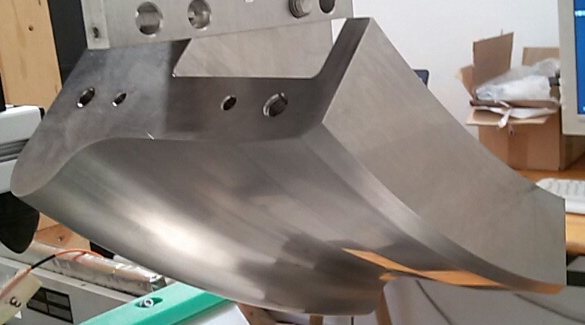
\includegraphics[width=\textwidth]{./images/analysis/exp2/DIMA.jpg}
    \caption{Photo of the DIMA}
    \label{fig:exp2-dima}
  \end{figure}
\vfill
  \begin{table}
\centering
\begin{tabular}{|c|c|c|c|c|}
\hline
\textbf{FH}   & \textbf{FT}   & \textbf{QR}   & \textbf{RW}   & \textbf{RT}   \\ \hline
\textit{(mm)} & \textit{(mm)} & \textit{(mm)} & \textit{(mm)} & \textit{(mm)} \\ \hline
$28.00$       & $32.52$       & $10.81$       & $135.01$      & $47.11$         \\ \hline
\end{tabular}
\caption{Measures of the DIMA}
\label{tab:exp2-measures}
\end{table}
\vfill
  \begin{figure}
    \centering
    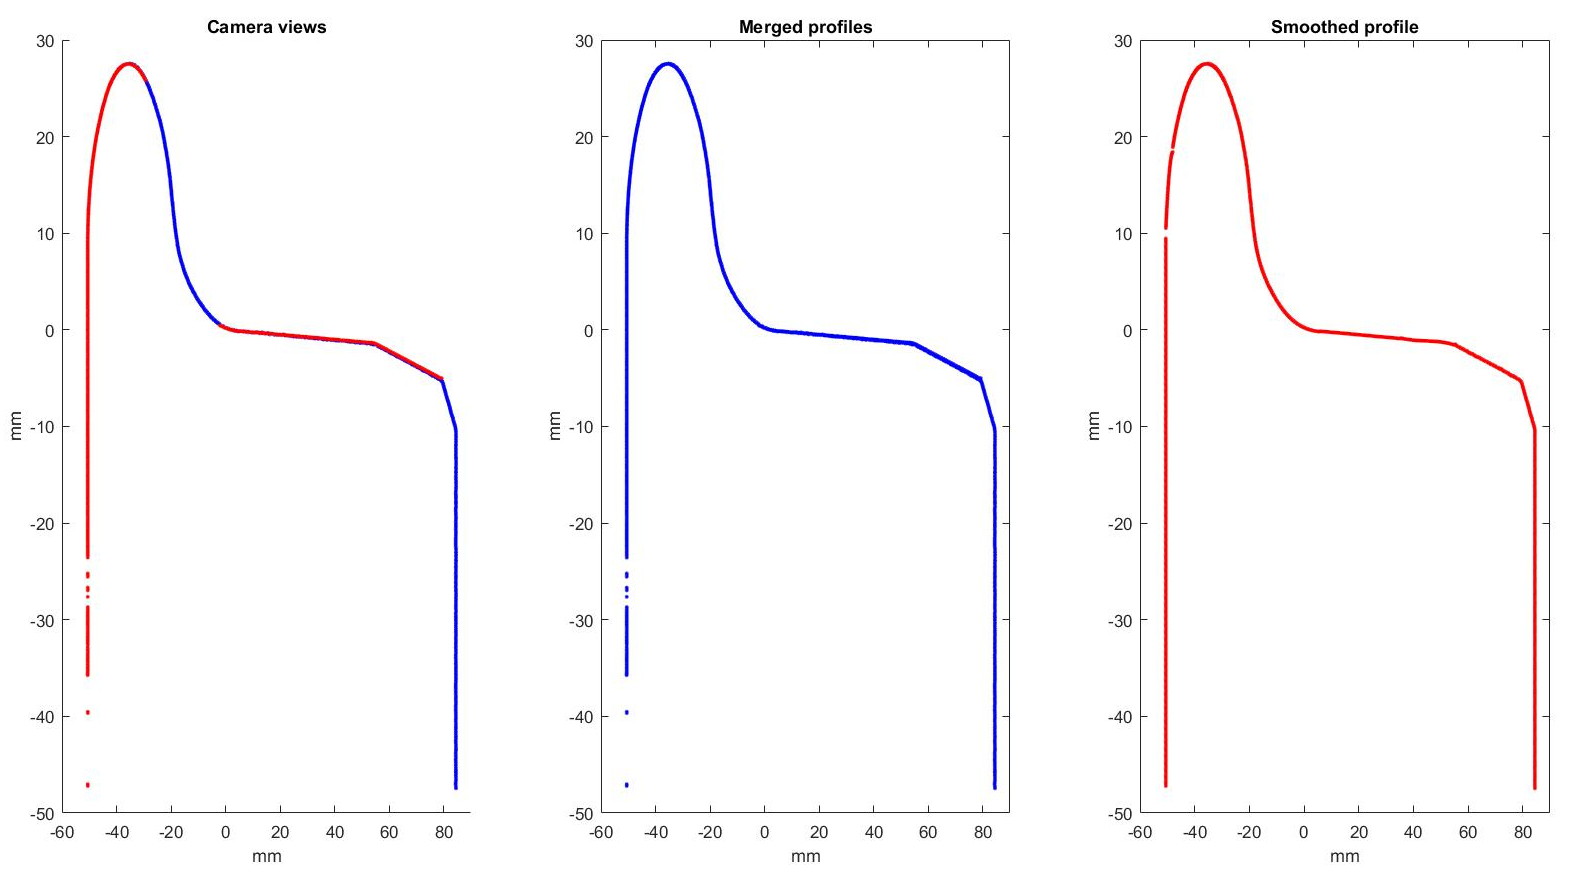
\includegraphics[width=\textwidth]{./images/analysis/exp2/wheel_steps.jpg}
    \caption{Steps used to merged the two profiles}
    \label{fig:exp2-merged}
  \end{figure}
\noindent
which used two different configurations, e.g. in terms of baselines length and triangulation angles. However, once again, all the parameters where comparable between the two algorithms, thus we continued with our analysis.

The second step, was the evaluation of the profile. Using the results of the previous set of experiments, we focused only on the \textit{center of mass}, \textit{Blais\&Rioux} and \textit{FIR} filters, ignoring the others. The windows used where of $16$ and $20$ pixels for each filter. After several attempts we correctly merged the two profiles collected by the two laser-camera pairs. To do that, we first converted the filtered laser in the world reference system, than we superimposed the two profiles and merged them in the same data structure. At the end we smoothed a bit the obtained profile, in order to reduce the effect of noise and the laser thickness, especially along the inner ad outer sides. The result reached is shown in Figure \ref{fig:exp2-merged}. \\

As shown in the last sub-plot, we had to pay attention when using \textsc{MatLab} functions: to increase the precision of this process, we decided to split the wheel's section in many parts, using the keypoints described above as extreme points of these curves; thus, we used a different mathematical model to smooth each part. During this process, it could happen that some gaps appear in the smoothed profile, reducing the precision of points location. As we will see, we can consider these errors negligible in our working conditions. \\

Finally, numerical results are shown. In Table \ref{tab:exp2:refereces} we reported an approximation of the errors committed at the center of the \acs{FOV}. It is already possible to see that, despite the improving given by the filters at pixel level, we haven't a same increase on the world reference system, i.e. in $mm$. Carefully analysing each step of the model, we noticed that the performance decreased on Equation \ref{eq:model:err:disc} and on Equation \ref{eq:det_a}. In the first case it is simple to understand why: the multiplication by the pixel size considerably reduces the weight of the error, especially if the pixel size is in the order of tenths of a millimiter. To be precise, this is not an error reduction, rather a change of scale, from pixel to millimeters; the smaller the pixel is, the smaller is the weight of the error. Regarding the second case, instead, we didn't find a good answer that can explain what happened. From our point of view, we could interpret this situation as an another change of reference system, from the camera to the world. However, the change of unit of measure was performed in case before. The only thing that can help us is that, a variation in the point in the space corresponds to a much smaller variation in the sensor, so the error is more apparent on the latter plane, rather than in the world.
  \begin{table}[h!]
  \centering
  \begin{tabular}{|l|r|r|r|r|}
    \hline
    \multirow{2}{*}{}  & \multicolumn{1}{c|}{\textbf{Approximation}} & \multicolumn{1}{c|}{\textbf{Y}}    & \multicolumn{1}{c|}{\textbf{X}}    & \multicolumn{1}{c|}{\textbf{Point error}} \\
	\hline
                       & \multicolumn{1}{c|}{\textit{(pixel)}}    & \multicolumn{1}{c|}{\textit{(mm)}} & \multicolumn{1}{c|}{\textit{(mm)}} & \multicolumn{1}{c|}{\textit{(mm)}}  \\
	\hline
    \textbf{Pixel}    & 0,4083    & 0,0353    & 0,0199    & 0,0405 \\
    \hline
    \textbf{CoM 16}   & 0,1877    & 0,0322    & 0,0195    & 0,0377 \\
    \hline
    \textbf{CoM 20}   & 0,1062    & 0,0316    & 0,0195    & 0,0372 \\
    \hline
    \textbf{BR 16}    & 0,1413    & 0,0319    & 0,0195    & 0,0374 \\
    \hline
    \textbf{BR 20}    & 0,1302    & 0,0318    & 0,0195    & 0,0373 \\
    \hline
    \textbf{FIR}      & 0,2587    & 0,0330    & 0,0196    & 0,0384 \\
    \hline
  \end{tabular}
  
  \caption{Reference values for propagation of the error (model output at the center of the \acs{FOV})}
  \label{tab:exp2:refereces}
\end{table}

Nevertheless, a comparison from theoretical and real results is shown in Table \ref{tab:exp2:means}. The values are the averages over the five measures mentioned above, evaluated using the points shown in Figure \ref{fig:exp2-cad}. As of the theoretical measures, they are estimated as differences between the values in column \textit{point error} of the Table \ref{tab:exp2:refereces}, but evaluated for the keypoints in figure. As we can see, the model is validated: the variation between theoretical and empirical results is comparable with the theoretical variance, so we can consider the results identical. There are only few consideration to take into account.
  \begin{table}[t!]
  \centering
  \begin{tabular}{|l|rr|rr|}
  \hline
  \multirow{3}{*}{} & \multicolumn{1}{c}{\textbf{\begin{tabular}[c]{@{}c@{}}Theoretical\\ Errors\end{tabular}}} & \multicolumn{1}{c|}{\textbf{Variance}} & \multicolumn{1}{c}{\textbf{\begin{tabular}[c]{@{}c@{}}Empirical\\ Errors\end{tabular}}} & \multicolumn{1}{c|}{\textbf{Variance}} \\
  \hline
  & \multicolumn{1}{c}{\textit{$(\mu m)$}}    & \multicolumn{1}{c|}{\textit{$(\mu m)$}}     & \multicolumn{1}{c}{\textit{$(\mu m)$}}    & \multicolumn{1}{c|}{\textit{$(\mu m)$}}     \\
  \hline
  \textbf{Pixel}     & 36.2    & 0.001400    & 105.1    & 5.9 \\
  \hline
  \textbf{CoM 16}    & 29.6    & 0.000973    & 32.1     & 0.5 \\
  \hline
  \textbf{CoM 20}    & 28.2    & 0.000823    & 33.5     & 0.7 \\
  \hline
  \textbf{BR 16}     & 28.8    & 0.000917    & 32.8     & 0.6 \\
  \hline
  \textbf{BR 20}     & 28.6    & 0.000875    & 30.0     & 0.4 \\
  \hline
  \textbf{FIR}       & 31.4    & 0.001240    & 29.6     & 0.3 \\
  \hline
  \end{tabular}
  
  \caption{Averages of the computed measures}
  \label{tab:exp2:means}
\end{table}

  \begin{figure}[t!]
    \centering
    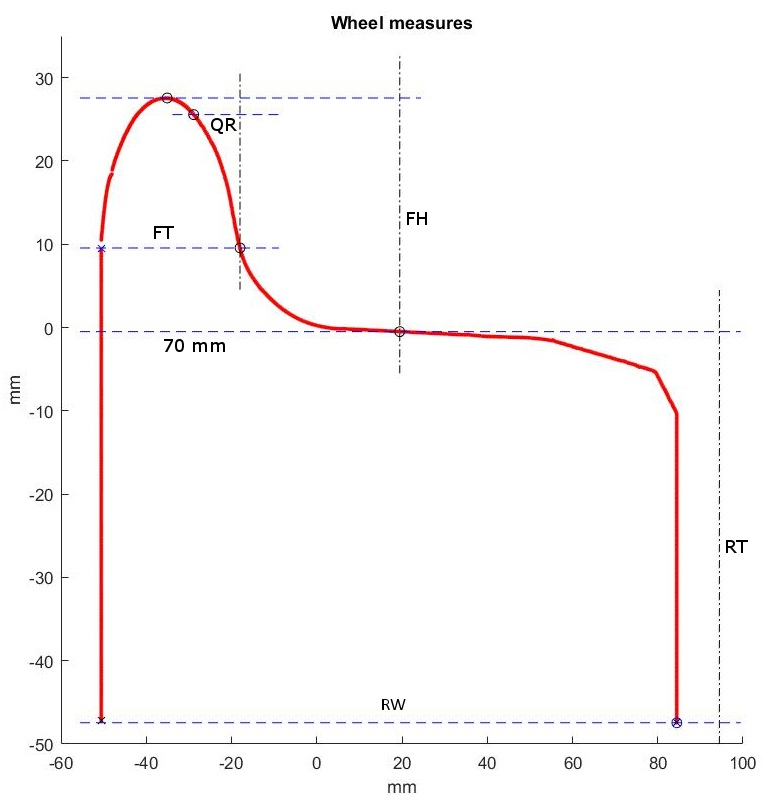
\includegraphics[width=0.88\textwidth]{./images/analysis/exp2/wheel_profile_mod.jpg}
    \caption{Analysed profile, with measure indication, CAD style.}
    \label{fig:exp2-cad}
  \end{figure}
As we said at the beginning of this section, we are using two laser-camera pairs, which results are merged to obtain the profile. The two systems used different configurations, in particular different triangulation angles and baselines. Despite this, differences are very small in terms of absolute values, we noticed that they lead to different output models, i.e. different error approximations. In Table \ref{tab:exp2:refereces}, as in the other phases of our analysis, the values in columns \textit{Y} and \textit{X} are the means of the two models. In this case we consider the means, instead of the error propagation for the variance in Equation \ref{eq:exp:var-prop}, because we didn't know to which piece of the profile the selected point belongs. Statistically, we had a probability of an half, thus we considered the mean as the most appropriate operator.

Another doubt we still had, regards the tuning of the model. Also in this case, we missed some informations, such as the precision of the Scheimpflug angle, or the orientation of the laser (it is a degree of freedom of the system). Thus, we needed to perform a tuning in order to balance the output with the empirical results. Notwithstanding the values used were reasonable with respect to the system structure, we thought that in this way, we mixed some errors due to the model and to the algorithm used to align and merge the two profiles. \\

To conclude, we can say that the model seems to be correct. This last set of tests allowed to underline the fact that it is a good approximation of the real scenarios, however, it has some degrees of freedom that must be analysed to get reasonable results. Also in this case, we remarked the importance of using windows comparable to the laser width, on the contrary the effects noise present in the acquired frames could be great enough to predominate on the laser. As far as the camera is concerned, we used here a sensor with pixels sizes smaller than the camera used in the previous section. As we can see, reducing pixels size reduces considerably the performances of the sub-pixel filters: this is reasonable if we think that a smaller pixel represents a smaller part of the world. \\
Two more considerations before continuing, concerning the resolution of the camera and the effects of noise in the frame. During our analysis we noticed that the empirical errors we obtained were very similar to the nominal resolution of the camera. This observation suggested us to control if a same thing happened in the previous set of experiments, and we noticed that it was quite true. Looking at the noise, however, we have noticed how to change the preprocessing of the image being analysed, changing the values of the empirical errors. More in-depth analyses are discussed in the sections bellow.
%
% Validation of the model
  \section{Validation of the model}
For the last set of tests, we returned over the initial optical bench. In this case, we wanted to compare the output of the model with the resolution of the camera, in order to understand if the precision of the measures we can make, is inferiorly limited by camera resolution, or if it is influenced also by some other factors. \\
To reach our goal, we decided to modify the bench a bit: we used a less distorted lens (the one used in the Section \ref{sec:exp1} introduced too much tangential distortion), and we changed the laser to a similar one to that used in Section \ref{sec:exp2}, less noisy and thick than the initial one (configuration in Table \ref{tab:conf3}). Thus, we calibrate the system again, using the company's software. At this point, we performed two different test:
 \begin{itemize}
   \item First, we repeated the experiments in Section \ref{sec:exp1}, using the same known target object.
   \item Second, we empirically evaluated the resolution of the camera, and compared the results with both the nominal value of the camera, and the results obtained in the first point.
 \end{itemize}
 \begin{table}
  \centering
  \begin{tabular}{ccccc}
  \hline
  \multicolumn{5}{|c|}{\textbf{Camera}}                                                                                                                                                                            \\ \hline
  \multicolumn{1}{|c|}{\textbf{Name}} & \multicolumn{1}{c|}{\textbf{Size}}      & \multicolumn{1}{c|}{\textbf{Pixel size}} & \multicolumn{1}{c|}{\textbf{Lens Manufacturer}} & \multicolumn{1}{c|}{\textbf{Focal}} \\ \hline
  \multicolumn{1}{|l|}{}              & \multicolumn{1}{c|}{\textit{pix x pix}} & \multicolumn{1}{c|}{\textit{mum}}        & \multicolumn{1}{c|}{}                           & \multicolumn{1}{c|}{\textit{mm}}    \\ \hline
  \multicolumn{1}{|l|}{Arya}          & \multicolumn{1}{c|}{4096 x 3072}        & \multicolumn{1}{c|}{5.5}                 & \multicolumn{1}{c|}{Shneider}                   & \multicolumn{1}{c|}{35}             \\ \hline
  \multicolumn{1}{l}{}                & \multicolumn{1}{l}{}                    & \multicolumn{1}{l}{}                     & \multicolumn{1}{l}{}                            & \multicolumn{1}{l}{}                \\ \cline{2-4}
  \multicolumn{1}{c|}{}               & \multicolumn{1}{c|}{\textbf{Laser}}     & \multicolumn{1}{c|}{}                    & \multicolumn{1}{c|}{}                           &                                     \\ \cline{2-4}
  \multicolumn{1}{c|}{}               & \multicolumn{1}{c|}{\textbf{Frequency}} & \multicolumn{1}{c|}{\textbf{Power}}      & \multicolumn{1}{c|}{\textbf{Aperture}}          &                                     \\ \cline{2-4}
  \multicolumn{1}{c|}{\textit{}}      & \multicolumn{1}{c|}{\textit{nm}}        & \multicolumn{1}{c|}{\textit{W}}          & \multicolumn{1}{c|}{\textit{degree}}            & \textit{}                           \\ \cline{2-4}
  \multicolumn{1}{c|}{}               & \multicolumn{1}{c|}{450}                & \multicolumn{1}{c|}{1.6}                 & \multicolumn{1}{c|}{45}                         &                                     \\ \cline{2-4}
  \end{tabular}

  \caption{Configuration of the third system.}
  \label{tab:conf3}
\end{table}

% --------- %
\subsection{Model validation}
In the first phase, the experiments were performed as described in Section \ref{sec:exp1}, but now we have limited the propagation of the errors to the single points, rather than proceeding with the measurements as before. Thus, we put the target in three know position: at the beginning, in the middle and at the end of the \acs{FOV}. This allowed us to cover the entire \acs{FOV} of the camera. In Table \ref{tab:exp3-res} we reported the obtained results. As before, the values are the means of the propagate error for each point over the same sub-filter. We repeated our analysis twice because, as we can see, in the first test, the target was taken in wrong positions. However, we reported all the results better to find some correlations with the results discussed in the next subsection. \\
  \begin{table}[b!]
\centering
\begin{tabular}{|l|l|r|r|r|l|l|l|l|}
\cline{1-1} \cline{3-5} \cline{7-9}
\multirow{3}{*}{} &  & \multicolumn{3}{c|}{\textbf{Test 1}}                                                                            &  & \multicolumn{3}{c|}{\textbf{Test 2}}                                                                            \\ \cline{3-5} \cline{7-9} 
                  &  & \multicolumn{1}{c|}{\textbf{Begin}} & \multicolumn{1}{c|}{\textbf{Center}} & \multicolumn{1}{c|}{\textbf{End}}  &  & \multicolumn{1}{c|}{\textbf{Begin}} & \multicolumn{1}{c|}{\textbf{Center}} & \multicolumn{1}{c|}{\textbf{End}}  \\ \cline{3-5} \cline{7-9} 
                  &  & \multicolumn{1}{c|}{\textit{(mm)}}  & \multicolumn{1}{c|}{\textit{(mm)}}   & \multicolumn{1}{c|}{\textit{(mm)}} &  & \multicolumn{1}{c|}{\textit{(mm)}}  & \multicolumn{1}{c|}{\textit{(mm)}}   & \multicolumn{1}{c|}{\textit{(mm)}} \\ \cline{1-1} \cline{3-5} \cline{7-9} 
\textbf{COM 16}   &  & 0.4320                              & 0.5635                               & 0.5915                             &  & 0.2997                              & 0.3211                               & 0.4247                             \\ \cline{1-1} \cline{3-5} \cline{7-9} 
\textbf{COM 20}   &  & 0.4322                              & 0.5638                               & 0.5910                             &  & 0.2798                              & 0.3212                               & 0.4247                             \\ \cline{1-1} \cline{3-5} \cline{7-9} 
\textbf{BR 16}    &  & 0.4322                              & 0.5642                               & 0.5917                             &  & 0.2800                              & 0.3216                               & 0.4251                             \\ \cline{1-1} \cline{3-5} \cline{7-9} 
\textbf{BR 20}    &  & 0.4322                              & 0.5644                               & 0.5636                             &  & 0.2800                              & 0.3217                               & 0.4251                             \\ \cline{1-1} \cline{3-5} \cline{7-9} 
\textbf{FIR}      &  & 0.4323                              & 0.5636                               & 0.5920                             &  & 0.2800                              & 0.3215                               & 0.4250                             \\ \cline{1-1} \cline{3-5} \cline{7-9} 
\end{tabular}
\caption{Error propagation to points, at the begin, the middle and the end of the \acs{FOV}}
\label{tab:exp3-res}
\end{table}
For the moment, the only consideration that we can make is the comparison with the results in Section \ref{sec:exp1}: the use of a less distorted lens, and the use of a better laser reduced significantly the theoretical error that we can commit.

% --------- %
\subsection{Camera resolution}
In the second phase, we decided to integrate our library with a method that allowed us to evaluate the resolution of the camera. To do that, we put the step motor, used to calibrate the system, parallel with the optical axis; in this way the reference object (used to create the grid of points required by Tsai) is perpendicular with the camera. In this case we are not interested in determining the edges of the object, but only to acquire a horizontal laser line. So, we saved six frames: two at the beginning of the \acs{FOV}, two in the middle, and two at the end; in each pair of the acquisitions, the laser lines are $5 \, mm$ apart. This value was chosen arbitrarily to appreciate the distance to the naked eye, and to be able to control the displacement between one position and the other with a tape measure. In Figure \ref{fig:line-pos} are shown the three positions of the target, with respect of the \acs{FOV} of the camera.
  \begin{figure}[!b]
    \centering
    \begin{minipage}[c]{.32\textwidth}
      \centering
      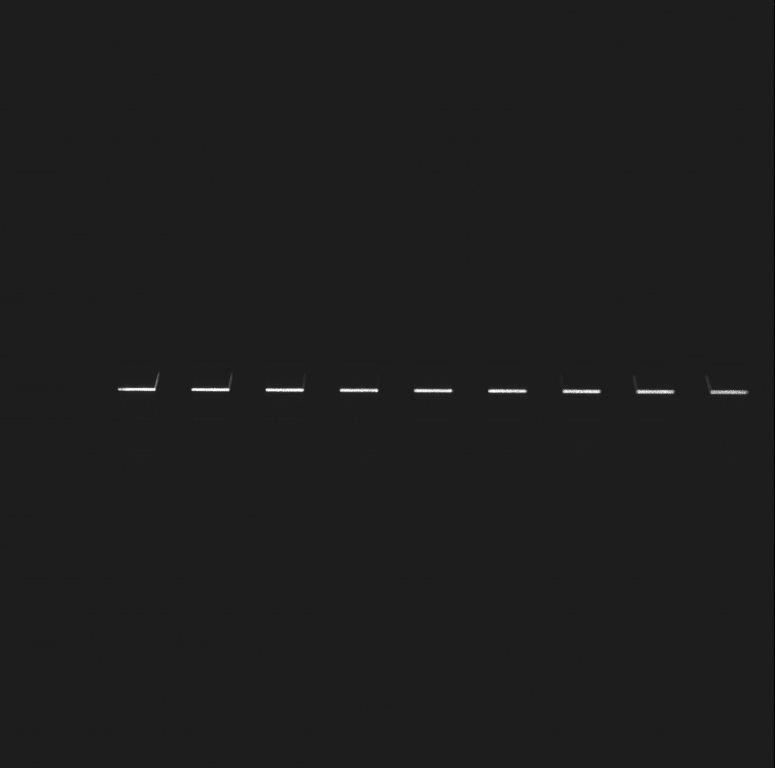
\includegraphics[width=\textwidth]{./images/analysis/exp3/250.jpg}
    \end{minipage}
    \hfill
    \begin{minipage}[c]{.32\textwidth}
      \centering
      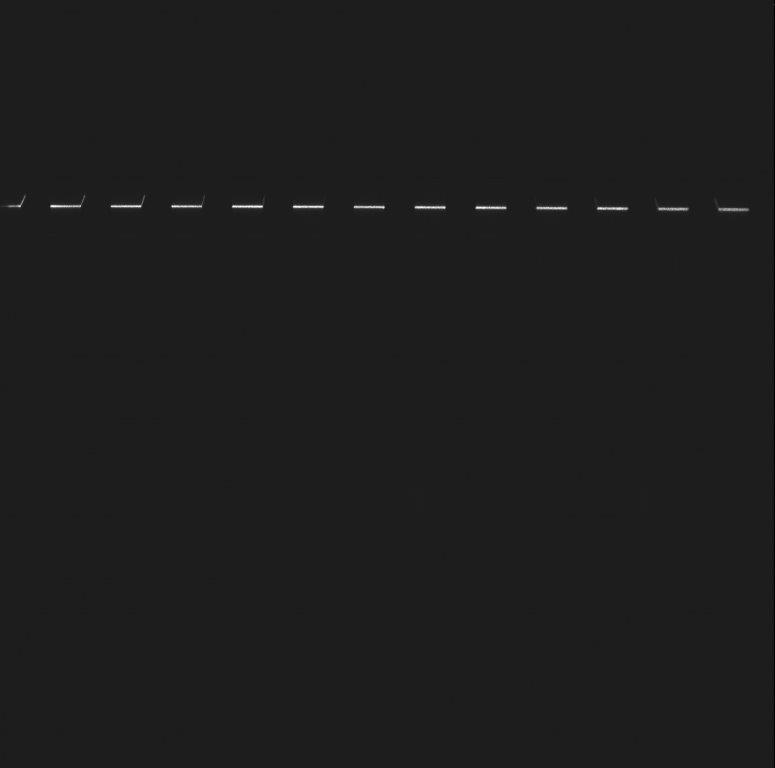
\includegraphics[width=\textwidth]{./images/analysis/exp3/380.jpg}
    \end{minipage}
    \hfill
    \begin{minipage}[c]{.32\textwidth}
      \centering
      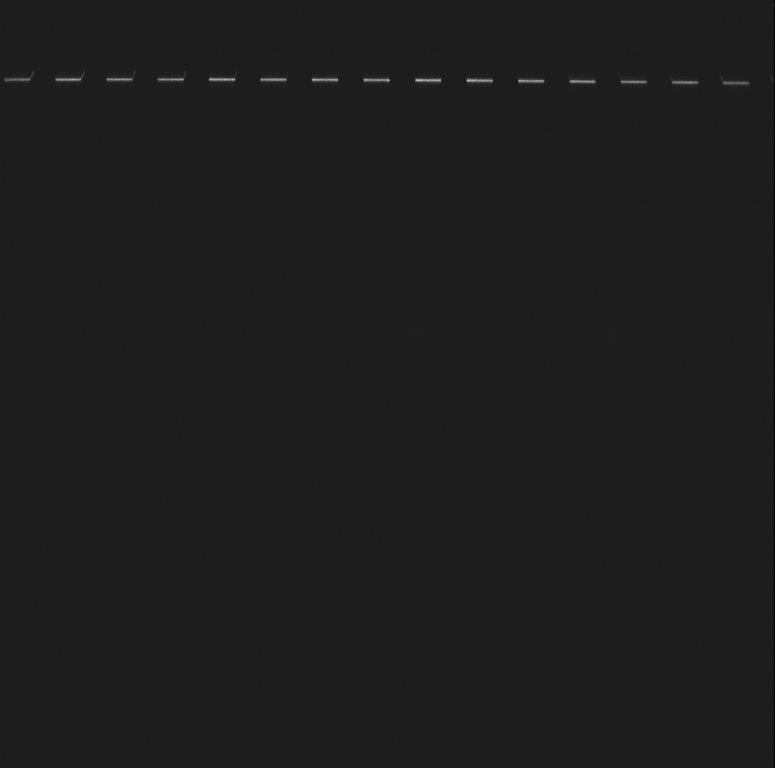
\includegraphics[width=\textwidth]{./images/analysis/exp3/510.jpg}
    \end{minipage}
    
    \caption{Positions of the target along the \acs{FOV} of the camera}
    \label{fig:line-pos}
  \end{figure}
In Table \ref{tab:exp3:res2} we reported our results: the first two columns are, respectively, the distances and the errors between the pairs of laser lines, while the third column contains the resolution of the camera, evaluated in the three position cited above. As we can see, the filters did not change resolutions substantially, so we can conclude that the resolution of our camera was in the range $\left( 0.27, 0.55 \right) \, mm/pix$. \\
  \begin{table}[t!]
  \centering
  \begin{tabular}{|cl|p{2.3cm}|p{2.3cm}|p{2.3cm}|}
  \hline
  \multicolumn{2}{|c|}{\multirow{2}{*}{}}              & \multicolumn{1}{c|}{\textbf{Mean}} & \multicolumn{1}{c|}{\textbf{Error}} & \multicolumn{1}{c|}{\textbf{Resolution}} \\
  \multicolumn{2}{|c|}{}                               & \multicolumn{1}{c|}{\textit{(mm)}} & \multicolumn{1}{c|}{\textit{(mm)}}  & \multicolumn{1}{c|}{\textit{(mm / pix)}} \\
  \hline
  \multirow{5}{*}{\textbf{Begin}}  & \textit{CoM 16} & 5,3318                            & 0,3318                             & 0,2730                                  \\
                                 & \textit{CoM 20} & 5,3333                            & 0,3333                             & 0,2731                                  \\
                                 & \textit{BR 16}  & 5,2878                            & 0,2878                             & 0,2730                                  \\
                                 & \textit{BR 20}  & 5,3176                            & 0,3176                             & 0,2731                                  \\
                                 & \textit{FIR}    & 5,3565                            & 0,3566                             & 0,2728                                  \\
  \hline
\multirow{5}{*}{\textbf{Center}} & \textit{CoM 16} & 5,6046                            & 0,6046                             & 0,4021                                  \\
                                 & \textit{CoM 20} & 5,5711                            & 0,5711                             & 0,4016                                  \\
                                 & \textit{BR 16}  & 5,7247                            & 0,7247                             & 0,4026                                  \\
                                 & \textit{BR 20}  & 5,6324                            & 0,6324                             & 0,4026                                  \\
                                 & \textit{FIR}    & 5,6177                            & 0,6177                             & 0,4028                                  \\
  \hline
\multirow{5}{*}{\textbf{End}}    & \textit{CoM 16} & 5,7494                            & 0,7494                             & 0,5500                                  \\
                                 & \textit{CoM 20} & 5,7647                            & 0,7647                             & 0,5501                                  \\
                                 & \textit{BR 16}  & 5,9726                            & 0,9726                             & 0,5504                                  \\
                                 & \textit{BR 20}  & 5,7809                            & 0,7809                             & 0,5510                                  \\
                                 & \textit{FIR}    & 6,3786                            & 1,3786                             & 0,5503                                 \\
    \hline
\end{tabular}
\caption{Camera resolution in \textit{mm/pix}, varying sub-pixel filter and location in the \acs{FOV}}
\label{tab:exp3:res2}
\end{table}

If we compare the values in Table \ref{tab:exp3-res} with the ones in Table \ref{tab:exp3:res2}, it is clear that the target wasn't acquired in the same positions, but despite that, we can say that the values are the same. From our point of view, this was an interesting result: if on the one hand, it has further validated the model, determining a physical lower bound that we have reached, on the other it confirmed what we said in Section \ref{sec:exp2} about the ``sensitive points'' of the model. In our case, the performances of the hardware were good enough to make the software's effects on the final results negligible. As we have already said, the smaller the pixel size is, the smaller the gain done by the filters.

% Noise effects
  \section{Noise effects}
To conclude our analysis, in the end we studied the behaviours of the sub-pixel filters varying the noise in the image. As we mentioned in Section \ref{sec:laser-peaks}, the presence of electrical noise in the frames \cite{1334612}, can affect heavily the quality of the peak detection, thus it is a good practice to apply some filters that reduce the weight of this noise during the laser location phase \cite{Naidu1991}. For example, industry experts know that such operations are necessary if you use the \textit{center of mass}: the presence of spikes influences the evaluation of the weighted average. An example of this, is shown in Figure \ref{fig:noise-es}. \\
  \begin{figure}[t!]
    \centering
    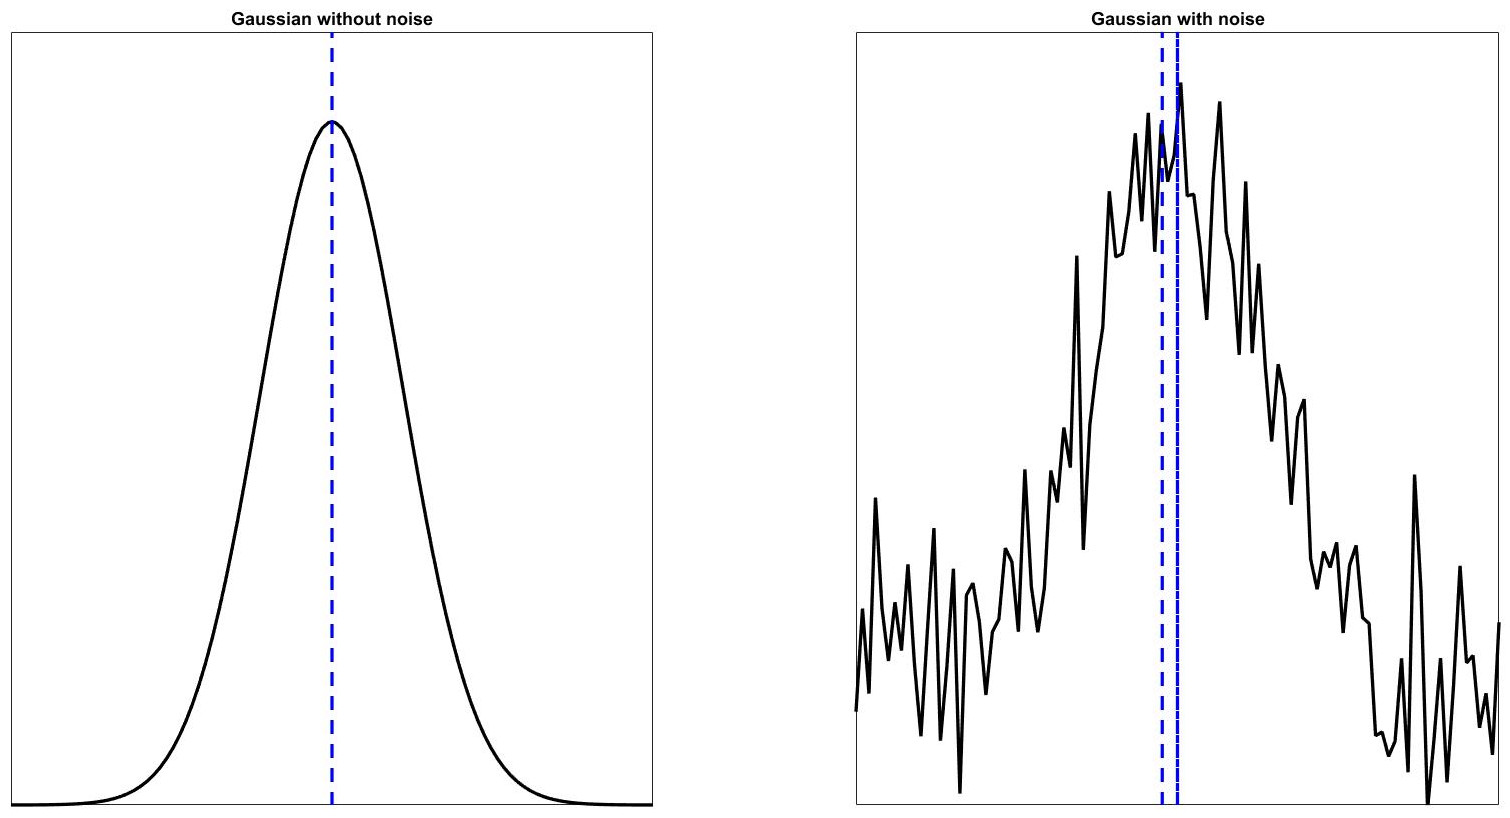
\includegraphics[width=\textwidth]{./images/analysis/noise/electrical.jpg}
    \caption{Effects of noise in peak detection. On the left there is a noise free Gaussian, and the \acs{COM} correctly detect the peak. On the right, the noise moves the location (-.) with respect to the correct one (- -).}
    \label{fig:noise-es}
  \end{figure}
  
As far as we are concerned, we have noticed these problems during the test shown in Section \ref{sec:exp2}. Before reaching the discussed results, we tried to apply different image preprocessing algorithms to increase the precision of the peak localizion. So we saw that when we changed the preprocessing, the final results changed too. In Figure \ref{fig:prep-dima} we reported the model trends for each sub-pixel filter used, varying the image preprocessing algorithms. As we can see, not all algorithms improve the results, on the contrary, sometimes they get worse the final error. In addition, we can see that the trend is different between mobile average and derivatives filters. These observations suggested us that not all filters have the same behaviour. Anyway, these results were obtained from a single system, thus we decided to perform some theoretical tests, in order to control the sources of noise. \\

In the second set of tests, we introduced some noise to the Gaussian, varying its \acs{SNR}. In this way we were able to see how much strong are the sub-pixel algorithms with respect to the noise, and thus to the variations in image conditions. To do that, we varied the \acs{SNR} in the range $\left( 0, 30 \right)$ with step $1$, and repeated the test five times per \acs{SNR} step. The averages of the results are shown in Figures \ref{fig:prep1} and \ref{fig:prep2}. We had to split the trends in two graphics to see better what happens. 

The first thing that caught our attention was the fact that, for high values of \acs{SNR}, the initial hypothesis that $\hat{\delta} \in \left( -\frac{1}{2}, \frac{1}{2} \right)$ with respect to the pixel, is false. The only model that always guarantees the hypothesis, is the \textit{FIR}. Unfortunately, we are not able to model this result mathematically. As we said in the previous chapters, the algorithm used to detects the peak, finds the pixel with the greater value along a row, and then applies on it the sub-pixel filters. If we think of a moment, this is a reasonable hypothesis: so we considered the possibility to go out from the pixel as an error due to the noise in the image.

The second important thing to underline, is the effect of the size of the window. As we have said several times, the window has to be comparable with the width of the Gaussian, however, in presence of noise, the bigger the window is, the bigger is the weight of the noise in the measure. We can see this for both \textit{center of mass} and \textit{B\&R}. Furthermore, in the same point we can notice that the \textit{FIR} filter, that is more robust than the others in presence of noise, becomes the worst. \\

Thus, we can conclude that, from a global point of view, the \textit{FIR} filter is the more robust in presence of noise, and it is the more stable, because of its small variance along noise variation. However, for low noise images \textit{center of mass} and \textit{B\&R} models, allow to reach better results. The \textit{B\&R} is the less stable filter, but as shown in Figure \ref{fig:prep-dima}, it is the less sensible (with the \textit{FIR} filter) to image preprocessing. Finally, as far as the window size is concerned, the rule on Gaussian dimension continues to apply. So, there isn't a filter better than the others: their behaviours strictly depends from the scenario we are working on, and from the preprocess applied to the image. Since these considerations are empirical, we suggest to perform some tests in real conditions before choosing what algorithm use in your application.
  \begin{figure}[b!]
    \centering
    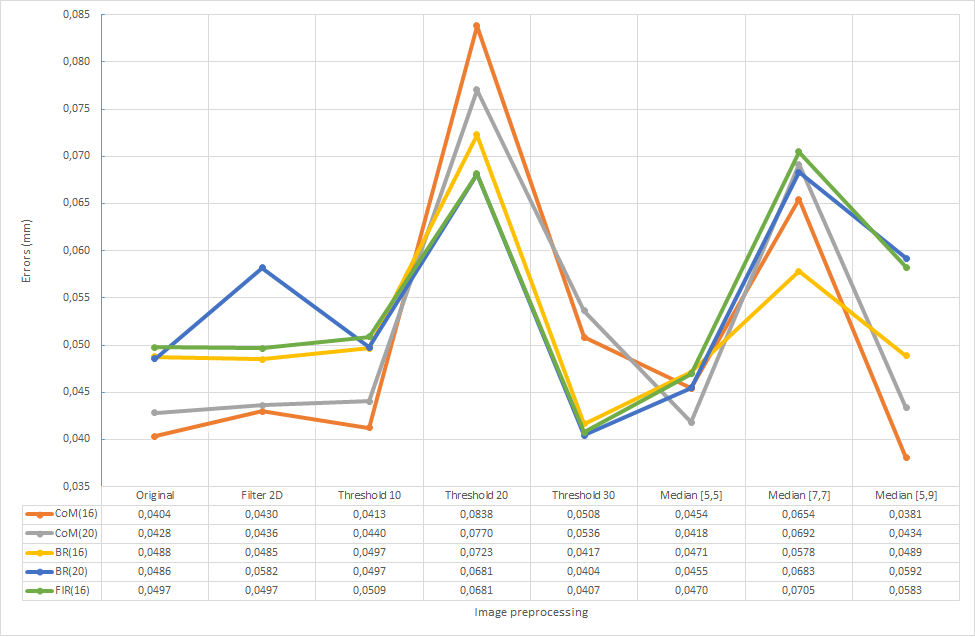
\includegraphics[width=0.95\textwidth]{./images/analysis/noise/preprocessing_dima.png}
    \caption{Variation in the model output changing the image preprocessing.}
    \label{fig:prep-dima}
  \end{figure}
\vfill
  \begin{figure}
    \centering
    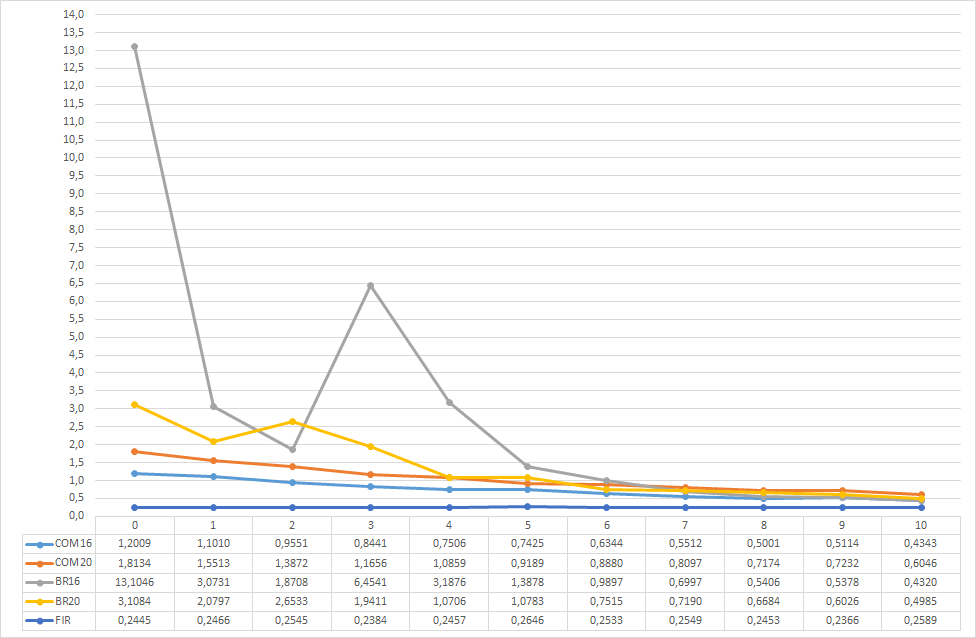
\includegraphics[width=\textwidth]{./images/analysis/noise/prep1.png}
    \caption{Filters' trends for \acs{SNR} in range $\left( 0, 10 \right)$}
    \label{fig:prep1}
  \end{figure}
\vfill
  \begin{figure}[t!]
    \centering
    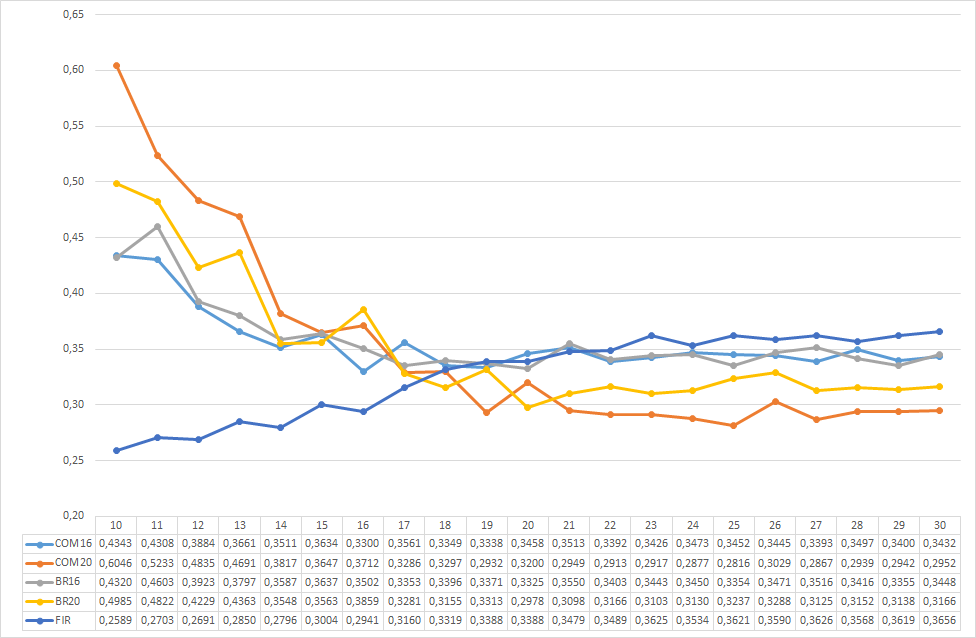
\includegraphics[width=\textwidth]{./images/analysis/noise/prep2.png}
    \caption{Filters' trends for \acs{SNR} in range $\left( 10, 30 \right)$}
    \label{fig:prep2}
  \end{figure}
  

%\textbf{COSE CHE HO VOLUTAMENTE LASCIATO INDIETRO}
%\begin{itemize}
%  \item Test sulla lente, che ha dimostrato che aveva qualche problema, perché il calibro mi veniva sinusoidale anziché parabolico
%\end{itemize}
